\documentclass[letterpaper,twocolumn,openany,nodeprecatedcode]{dndbook}
\usepackage{amsmath}
\usepackage[english]{babel}
\usepackage[utf8]{inputenc}
\usepackage[singlelinecheck=false]{caption}
\usepackage{lipsum}
\usepackage{listings}
\usepackage{shortvrb}
\usepackage{stfloats}
\usepackage{graphicx}
\usepackage[inkscapelatex=false]{svg}
\usepackage{hyperref}
\usepackage{tcolorbox}
\tcbuselibrary{skins, breakable}
\usepackage{enumitem}
\usepackage{hyperref}

\usepackage{svg}
\svgsetup{inkscapeexe=inkscape}
\usepackage{pdflscape}
\usepackage{graphicx}
\usepackage{circuitikz}
\usetikzlibrary{positioning} % Additional library for relative positioning 
\usetikzlibrary{calc} % Additional library for calculating within tikz
\usetikzlibrary{shapes.geometric, arrows}

\usetikzlibrary{arrows.meta, positioning}

\usetikzlibrary{circuits.logic.US, positioning}


%--- Custom Colors ---
\definecolor{aliceblue}{RGB}{230, 240, 255}
\definecolor{alicetext}{RGB}{0, 50, 150}
\definecolor{bobgreen}{RGB}{235, 255, 235}
\definecolor{bobtext}{RGB}{0, 100, 50}
\definecolor{conceptgray}{RGB}{245, 245, 245}

%--- Custom Box Definitions ---

% Box for Alice (Transmitter)
\newtcolorbox{alicebox}[1]{
    colback=aliceblue,
    colframe=alicetext,
    fonttitle=\bfseries\Large,
    coltitle=white,
    title={#1},
    enhanced,
    attach boxed title to top left={xshift=5mm, yshift=-2mm},
    boxed title style={colback=alicetext, sharp corners},
    sharp corners=south,
    arc=5mm
}

% Box for Bob (Receiver)
\newtcolorbox{bobbox}[1]{
    colback=bobgreen,
    colframe=bobtext,
    fonttitle=\bfseries\Large,
    coltitle=white,
    title={#1},
    enhanced,
    attach boxed title to top right={xshift=-5mm, yshift=-2mm},
    boxed title style={colback=bobtext, sharp corners},
    sharp corners=south,
    arc=5mm
}

% Box for Key Concepts
\newtcolorbox{conceptbox}[1]{
    colback=conceptgray,
    colframe=black!60,
    fonttitle=\bfseries,
    title={#1},
    leftrule=4pt,
    arc=2mm
}

\captionsetup[table]{labelformat=empty,font={sf,sc,bf,},skip=0pt}

\MakeShortVerb{|}

\lstset{%
  basicstyle=\ttfamily\small,
  language=C,
  breaklines=true,
  frame=single,
  numbers=left,
  numberstyle=\tiny,
}

\newcommand{\ChapterCredits}[1]{%
\vspace{1em}
\begin{DndReadAloud}
  \textbf{Committed to parchment by:} #1
\end{DndReadAloud}
\vspace{1em}
}

\title{SDR Grimoire\\
\large A Comprehensive Manual for Practical Communications using SDR and USRP}
\author{Comm Lab Students}
\date{\today}

% Set theme color for SDR manual (using a tech-appropriate color)
\DndSetThemeColor[PhbLightCyan]

\begin{document}

\frontmatter

\maketitle

\tableofcontents

\mainmatter
\chapter*{Contributions}
\addcontentsline{toc}{chapter}{Contributions}

This grimoire was a collaborative effort. The following list documents primary contributors
to each chapter.

\section*{Chapter Contributions}

\begin{itemize}[leftmargin=1.5em]

\item \textbf{Pluto Hardware Architecture}  
Primary authors: Mihir Divyansh E, Vemula Siddhartha 

\item \textbf{Buffer Architecture and Digital Data Flow}  
Primary authors: Mihir Divyansh E, Vemula Siddhartha 

\item \textbf{MATLAB Programming Interface}  
Primary authors: Mihir Divyansh E, Vemula Siddhartha 

\item \textbf{Digital Communications Example}  
Primary authors: Mihir Divyansh E, Vemula Siddhartha  

\item \textbf{Digital Communications Exercises}  
Primary authors: Mihir Divyansh E, Vemula Siddhartha  

\item \textbf{USRP B210 Projects}
Primary authors: Dhanush V Nayak, Kaustubh Khachane

\item \textbf{Cross-Platform Comms}
Primary authors: Dhanush V Nayak, Kaustubh Khachane

\item \textbf{USRP X310 Architecture}  
Primary authors: Prabhat Kukunuri, H Anantha Krishnan, Varun Shakunaveti
Reference validation: Vendor Documentation  

\item \textbf{Python-Based SDR Examples}  
Primary authors: Prabhat Kukunuri, H Anantha Krishnan, Varun Shakunaveti
Integration testing: Comm Lab Students  

\item \textbf{Threading and Concurrency in SDR}  
Primary authors: Mihir Divyansh E, Vemula Siddhartha  

\item \textbf{Appendices and Reference Tables}  
Compiled by: Everyone 

\end{itemize}

\begin{DndReadAloud}
This document reflects collective effort. Any errors remain the responsibility of the authors.
\end{DndReadAloud}


\chapter{Pluto Architecture}
\ChapterCredits{
  Mihir Divyansh E,
  Vemula Siddhartha
}

\section{Hardware Transmit and Receive Signal Paths}

Figure~\ref{fig:plutofe} illustrates the complete RF front-end signal chain of the PlutoSDR, from digital baseband samples to the RF antenna interface and vice versa. This section describes the end-to-end transmit (TX) and receive (RX) paths at the hardware level.

\begin{figure*}[h]
  \centering
  \includesvg[width=0.95\linewidth]{figs/plutofe.svg}
  \caption{PlutoSDR RF front-end architecture}
  \label{fig:plutofe}
\end{figure*}

\subsection{Transmit Signal Path (Baseband Buffer to Antenna)}

The transmit signal path begins with complex baseband samples generated either on the host computer (e.g., MATLAB, GNU Radio) or internally within the PlutoSDR processing system. These samples are transferred to the PlutoSDR over USB and written into transmit buffers managed by the Zynq processing system.

From this point onward, the signal path is entirely hardware-driven.

\paragraph{Digital Baseband Interface}
Baseband samples are delivered to the AD9361 transceiver via a dedicated digital interface between the Zynq programmable logic and the transceiver. The samples are represented as interleaved, signed 12-bit I/Q values at the selected baseband sample rate.

\paragraph{Digital Interpolation and Filtering}
Inside the AD9361, the baseband samples pass through a configurable digital interpolation chain. This stage performs:
\begin{itemize}
  \item Sample rate conversion to match the RF front-end clocking
  \item Digital low-pass filtering to shape the transmitted spectrum
\end{itemize}

The interpolation factor is automatically configured based on the requested baseband sample rate and RF bandwidth.

\paragraph{Digital-to-Analog Conversion}
The filtered digital samples are converted into analog I and Q waveforms using 12-bit DACs. These DACs operate at a much higher internal clock rate than the input baseband sample rate, as set by the interpolation stages.

\paragraph{Analog Baseband and RF Upconversion}
The analog I/Q signals pass through baseband reconstruction filters and programmable gain/attenuation stages before entering the quadrature RF mixer. The mixer performs upconversion using the on-chip local oscillator (LO), translating the baseband signal to the configured RF center frequency.

\paragraph{RF Output Chain}
After upconversion, the RF signal passes through:
\begin{itemize}
  \item Programmable RF attenuators
  \item On-chip RF filters
  \item A low-power RF driver amplifier
\end{itemize}

The final RF signal is routed to the transmit SMA connector. The maximum achievable output power is limited by the on-chip RF driver stage and is typically on the order of a few (5-7) dBm into a 50~\(\Omega\) load.

\subsection{Receive Signal Path (Antenna to Baseband Buffer)}

The receive signal path mirrors the transmit chain in reverse order, beginning at the RF input connector and ending with digital baseband samples delivered to memory buffers in the processing system.

\paragraph{RF Input and Front-End Conditioning}
Incoming RF signals enter through the RX SMA connector and are first passed through on-chip RF filters and programmable gain stages. These stages provide coarse gain control and out-of-band interference rejection.

\paragraph{RF Downconversion}
The conditioned RF signal is mixed with a locally generated LO inside the AD9361, converting the signal from the RF center frequency down to complex baseband. The I and Q components are produced by a quadrature mixer.

\paragraph{Analog Baseband Filtering and Gain Control}
The downconverted I and Q signals pass through analog low-pass filters and variable gain amplifiers. These stages determine the effective noise figure and dynamic range of the receiver and are configured automatically or manually depending on the selected gain mode (manual or AGC).

\paragraph{Analog-to-Digital Conversion}
The analog baseband signals are sampled by 12-bit ADCs at high internal clock rates. The ADC output represents the digitized I/Q baseband signal prior to any decimation.

\paragraph{Digital Decimation and Filtering}
The digitized samples pass through a digital decimation chain inside the AD9361, which:
\begin{itemize}
  \item Reduces the sample rate to the user-configured baseband rate
  \item Applies digital low-pass filtering to limit noise and aliasing
\end{itemize}

As with transmission, the decimation factor is automatically determined by the selected baseband sample rate and RF bandwidth.

\paragraph{Baseband Data Delivery}
The final complex baseband samples are streamed from the AD9361 to the Zynq processing system and stored in receive buffers. 

\subsection{Notes on Symmetry and Shared Resources}

The transmit and receive chains share several common resources within the AD9361, including:
\begin{itemize}
  \item Local oscillator generation and frequency synthesis
  \item Clocking infrastructure
  \item Digital filter configurations
\end{itemize}

As a result, changes to parameters such as sample rate, RF bandwidth, or LO frequency can affect both TX and RX behavior, even when only one direction is actively used.

\begin{DndReadAloud}
  Understanding the hardware signal path is essential for diagnosing practical issues. Many apparent ``software problems'' originate from misconfigured hardware stages within the transmit or receive chains. Along with this, this understanding is important for realising practicality of any undertaking. 
\end{DndReadAloud}


\subsection{Dual Transmit and Receive Channel Operation}

The AD9361 transceiver used in the PlutoSDR internally supports two independent transmit (TX1, TX2) and two independent receive (RX1, RX2) signal chains. These channels are structurally symmetric and largely identical in terms of analog, mixed-signal, and digital processing blocks, as illustrated in Fig.~\ref{fig:plutofe}. However, in the stock PlutoSDR configuration, only one transmit and one receive channel are routed to external RF connectors.
The 2 TX paths have common clocking, and control, which ensure coherent operation, similar with 2RX

\paragraph{Practical Implications}
Although the AD9361 supports true 2T2R operation, enabling both channels simultaneously increases internal data throughput and places additional load on downstream data movement and buffering mechanisms. Furthermore, shared RF resources such as synthesizers and calibration engines mean that configuration changes to one channel can have side effects on the other.


\section{Exercises}

The questions are supposed to help you understand the architecture better, so you can make better sense of why something happens. They are not designed to have short or purely factual answers. Instead, you are encouraged to reason through the signal path, identify relevant hardware blocks, and—where possible—validate their conclusions experimentally.

\subsection*{Signal Path Awareness}

\begin{enumerate}
  \item For each of the following configuration parameters, identify the earliest hardware block at which the change takes effect. Refer to Fig \ref{fig:plutofe}
  \begin{itemize}
    \item Baseband sample rate
    \item RF bandwidth
    \item TX gain / attenuation
    \item RX gain (manual versus AGC)
  \end{itemize}

  \item A baseband waveform is transmitted at 1~MSPS and then retransmitted at 2~MSPS while keeping the RF bandwidth constant. Which internal stages must reconfigure, and what changes would you expect to observe at the RF output?
\end{enumerate}

\subsection*{Shared Resources}

\begin{enumerate}
  \setcounter{enumi}{2}
  \item If the TX center frequency is suddenly changed while operating in RX-only mode, what do you expect to see on the RX side?

  \item While receiving a continuous signal, the RX bandwidth is modified. Which internal blocks are affected by this change, and how would this affect the received signal? Think about before the switch, around the switch, and after the switch. If possible, draw crude waveforms (time domain i/q, spectrum), by studying the datasheet in \cite{AD9361_UG570}
\end{enumerate}

\subsection*{Dual-Channel Operation}

\begin{enumerate}
  \setcounter{enumi}{4}
  \item The two transmit chains share a common clock and local oscillator. List experiments that benefit from this coherence. For each experiment, identify which hardware block(s) would reveal loss of coherence first.
\end{enumerate}

\subsection*{Debugging and Fault Localization}

\begin{enumerate}
  \setcounter{enumi}{5}
  \item Unexpected spectral images are observed at the RF output. List three plausible causes and identify whether each originates in the digital baseband, analog baseband, or RF stages.

  \item A received signal becomes distorted only when RX gain is adjusted rapidly. Is this issue more likely rooted in RF hardware behavior, digital signal processing, or software interaction? Justify your reasoning.
\end{enumerate}

\subsection*{Architectural Limits}

\begin{enumerate}
  \setcounter{enumi}{8}
  \item Consider an application that requires transmit and receive samples to be aligned within 1~\(\mu\)s. Which aspects of the PlutoSDR architecture impose the strongest limitations on achieving this requirement? How do you propose you can circumvent this by the custom C library method? Design a software architecture, to achieve this on zynq

  \item You are allowed to modify only one layer of the system (host software, processing system software, programmable logic, or RF configuration). Which layer would you choose to most effectively reduce latency, and which to improve determinism? Explain your choices.
\end{enumerate}

\begin{DndReadAloud}
  If thou cannot clearly identify wh're a signal is delayed, filtered, or re-timed, thou art not eft to command it.
\end{DndReadAloud}


\chapter{Digital Data Flow}
\ChapterCredits{
  Mihir Divyansh E,
  Vemula Siddhartha
}

\section{Overview}

In the PlutoSDR, buffering appears at multiple boundaries: inside the RF transceiver, within the FPGA fabric, across the processor subsystem, and finally at the USB interface to the host computer. Understanding this multi$-$level buffer hierarchy is essential to understand synchronisation limits, update dynamics, and more importantly feasibility of any given project involving SDR. 

\begin{DndReadAloud}
    No, seriously, a lot of what you can and cannot do, depends on the buffering semantics, as this is a considerable portion of the latency.
\end{DndReadAloud}
This chapter describes the buffer architecture of the PlutoSDR from the lowest hardware level to the host interface, focusing on how samples move through the system and where bottlenecks can arise.
\section{The Role of Buffers}

Buffers are temporary storage regions that hold data as it moves between different processing stages or across interface boundaries. In streaming systems such as SDRs, buffers solve a fundamental problem: while RF hardware operates continuously in real time, software processing and data transport are inherently bursty and subject to unpredictable delays.

By introducing elasticity into the data path, buffers:
\begin{itemize}
  \item Absorb short$-$term timing variations between producers and consumers
  \item Allow components operating in different clock domains to interact safely
  \item Enable batch$-$based data transfers across inefficient interfaces such as USB
\end{itemize}

Without buffering, even momentary delays in software execution would immediately cause data loss. With insufficient buffering, reliable sustained operation at high sample rates becomes impossible.

\section{Buffer Hierarchy}

The PlutoSDR implements buffering at several distinct layers, each aligned with a physical or logical boundary in the system. These layers differ in size, function, and level of user visibility.

\subsection{AD9361 Internal Buffers}

At the lowest level, the AD9361 RF transceiver contains small internal FIFOs that sit between the high$-$speed ADCs and DACs and the digital filtering and interpolation/decimation stages. These buffers are entirely internal to the transceiver and are not directly configurable by the user.

Their primary purpose is to support interpolation and decimation without interrupting real$-$time sampling

On the receive path, samples accumulate after ADC conversion and digital decimation before being transferred out of the transceiver. On the transmit path, samples must be available in sufficient quantity ahead of DAC conversion to prevent underruns. Because these buffers are small, they provide only minimal tolerance to timing disturbances.

\subsection{Programmable Logic (PL) Buffers}

Above the AD9361 lie buffers implemented within the Zynq programmable logic (PL). These are typically realized using FPGA block RAM configured as FIFOs.

PL$-$side buffers serve several critical roles:

\begin{itemize}
  \item \textbf{Clock domain crossing:} The AD9361 operates on clocks derived from the RF subsystem, while the Zynq processing system uses different clock domains. Asynchronous FIFOs are used here for crossing.
  \item \textbf{Rate smoothing:} Short$-$term fluctuations in Processing System response—due to interrupts, bus contention, or scheduling—are absorbed without disrupting the RF data stream.
  \item \textbf{Data width conversion:} The AD9361 produces 12$-$bit I/Q samples, while the internal system buses typically operate on wider word sizes.
\end{itemize}

These buffers are relatively small, typically holding on the order of hundreds to a few thousand samples. They are designed to absorb brief timing mismatches rather than to store large amounts of data.

\subsection{Processing System (PS) Buffers}

Once data crosses from the PL into the Zynq Processing System, buffering transitions from hardware$-$managed to software$-$managed. Samples are stored in DDR memory buffers allocated by the Linux Industrial I/O (IIO) subsystem.

PS$-$side buffers are significantly larger than PL buffers and are typically implemented as circular buffers capable of holding tens of thousands of samples. Their size and behavior are configurable through software.

These buffers serve several important functions:

\begin{itemize}
  \item \textbf{USB transfer efficiency:} USB transfers are inefficient for small payloads. Large buffers allow the system to batch data into fewer, larger transfers.
  \item \textbf{Timing isolation:} Software delays on either the PlutoSDR or host side do not immediately impact the real$-$time RF hardware.
  \item \textbf{Computation staging:} When signal processing is performed on the PlutoSDR itself, these buffers provide working memory for block$-$based algorithms.
\end{itemize}

While PS buffers provide substantial elasticity, they also introduce latency that must be considered in time$-$sensitive applications.

\subsection{USB DMA and Host Transfer}

The final stage in the data flow involves Direct Memory Access (DMA) between PS buffers and the USB controller, followed by USB bulk transfers to the host computer.

On the transmit path, IQ samples flow from the host to PS memory via USB, then onward through the PL and into the AD9361. On the receive path, samples move in the opposite direction, accumulating in PS buffers until transferred to the host.

Although USB 2.0 advertises a theoretical throughput of 480~Mbps, sustained usable bandwidth is lower due to protocol overhead and host$-$side limitations. For high sample rate operation, USB bandwidth often becomes the dominant performance bottleneck, making careful buffer sizing and rate management essential.

\section{Underruns and Overruns}

Buffering failures generally appear in one of two forms:

\begin{itemize}
  \item \textbf{Transmit underruns}, where the RF hardware consumes samples faster than they are supplied, resulting in repeated or zero$-$valued samples and visible spectral artifacts.
  \item \textbf{Receive overruns}, where incoming samples arrive faster than they can be consumed, forcing the system to discard data and creating gaps in the received signal stream.
\end{itemize}

Both conditions arise from sustained rate mismatches rather than brief timing anomalies. Buffers can absorb short$-$term disruptions, but no buffer can compensate if the average data rate exceeds what downstream components can handle.

\section{Buffer Size Tradeoffs}

Increasing buffer sizes improves tolerance to timing variations and reduces the likelihood of underruns and overruns, but at the cost of increased latency. Every additional buffer stage adds delay between RF sampling and sample availability at the host.

Applications with strict latency requirements must operate with smaller buffers and accept a higher risk of data loss. Applications focused on recording or offline analysis can use larger buffers to maximize reliability.
\begin{DndReadAloud}
  In the PlutoSDR, most high$-$sample$-$rate failures are not caused by misconfigured RF parameters but by mismatches between buffer capacity, USB bandwidth, and software execution timing. Understanding the buffer hierarchy is therefore central to diagnosing performance problems.
\end{DndReadAloud}

\section{Implications for Timing$-$Critical Applications}

The layered buffer architecture described above has direct and unavoidable consequences for applications requiring tight timing control. While the PlutoSDR is highly flexible in terms of signal generation and capture, it is fundamentally not a low$-$latency, tightly synchronized RF platform. This section explains why certain classes of applications—most notably fast adaptive transmission and radar systems—are impractical or infeasible on the PlutoSDR.

\subsection{Limits on Fast Transmit Buffer Switching}

In adaptive communication systems, it is often desirable to switch transmit waveforms or parameters accurately on very short timescales (e.g., below a few (4)~ms, near coherence time), based on channel feedback or receiver measurements. Examples include fast link adaptation, burst$-$based protocols, or time$-$slotted systems.

On the PlutoSDR, transmit data originates on the host computer and must traverse the following stages before reaching the RF hardware:
\begin{enumerate}
  \item Host OS scheduling overhead
  \item Host$-$side application buffers
  \item USB transfer buffers
  \item Device OS scheduling overhead
  \item Processing System (PS) memory buffers
  \item PL$-$side FIFOs
  \item AD9361 internal buffers
\end{enumerate}

Each stage in the data path introduces both latency and timing uncertainty. USB transfers occur in burst$-$oriented transactions rather than at continuous sample granularity, Linux scheduling adds non$-$deterministic delays, and the large buffers in the Processing System are deliberately designed to decouple software execution from real$-$time RF operation. As a result, actions taken by the host application—such as switching to a new transmit buffer—are separated from RF emission by multiple layers of buffering and cannot be mapped to a precisely defined transmit time.

Under typical operating conditions, this delay is on the order of milliseconds and varies with system load and buffer configuration. Consequently, reliable transmit buffer switching on sub$-$10~ms timescales is not achievable when the PlutoSDR is driven from a host computer over USB. Operating in this regime generally produces delayed or uneven transitions and non$-$repeatable timing behavior, rather than deterministic, tightly bounded updates.

\subsection{Transmit$-$$-$Receive Synchronization Constraints}

Radar systems and certain sensing applications impose far stricter timing requirements than most communication systems. In pulse radar or FMCW radar, accurate detection depends on precise knowledge of the timing relationship between transmitted and received signals. This often requires:
\begin{itemize}
  \item Deterministic transmit start times
  \item Known and stable latency between TX and RX paths
  \item Sample$-$level or microsecond$-$level synchronization
\end{itemize}

Although the AD9361 itself is capable of coherent transmit and receive operation with shared clocks and local oscillators, this determinism does not extend across the full PlutoSDR system. Once samples pass beyond the RF transceiver into the PL and PS buffer layers, timing becomes software$-$mediated and non$-$deterministic.

On the receive side, samples that are captured at a precise RF time are delivered to the host only after traversing multiple buffering stages. On the transmit side, samples are emitted by the RF hardware based on when the internal buffers are filled, not on when the host application issues a command. There is no hardware mechanism on the PlutoSDR to align a specific transmit sample boundary with a specific received sample boundary in host$-$visible time.

As a result, while you can post$-$process received data and observe returns, accurately relating these samples to the precise transmit event that caused them is not possible with tight timing guarantees.

We can do multiple TX antennas to establish the reference transmit stream, and measure the reflection, but this has problems concerning the resolution achievable being $>6$m at optimal conditions

\subsection{What the PlutoSDR \emph{Can} Do Instead}

These limitations do not imply that the PlutoSDR is unsuitable for experimentation or learning. Rather, we can define the regime in which the platform operates well.

The PlutoSDR is well$-$suited for:
\begin{itemize}
  \item Continuous or quasi$-$continuous transmission and reception.
  \item Spectral analysis and waveform experimentation
  \item Slow adaptation on timescales of hundreds of milliseconds or more
  \item Understanding the problems faced in communications, beyond textbook
\end{itemize}

Applications requiring tight real$-$time control, deterministic latency, or microsecond$-$level synchronization generally require SDR platforms with FPGA$-$resident processing, direct RF triggering, and high$-$speed host interfaces (e.g., PCIe instead of USB).
It can also be done, as an exercise for interested readers, by creating your own library in C, cross compiling to ARM Cortex cores, and running the system natively on the SoC, but this of course has compute constraints, but nevertheless is good for control heavy tasks such as fast adaptation

\section*{Exercises}

\subsection*{Buffering and Latency}

\begin{enumerate}
  \item Identify all buffer stages that a receive sample traverses between the ADC in the AD9361 and availability to a host$-$side application. For each stage, indicate whether it primarily adds latency, variability, or throughput efficiency.

  \item Consider a receive configuration operating at 4~MSPS with a processing$-$system buffer depth of 65{,}536 samples. What is the minimum buffering latency introduced by this buffer alone? How does this compare to RF propagation delays?
\end{enumerate}

\subsection*{USB and Operating System Effects}

\begin{enumerate}
  \setcounter{enumi}{2}
  \item USB bulk transfers are optimized for throughput rather than latency. Explain how this affects determinism in SDR streaming applications.

  \item Suppose a host application delivers transmit buffers at perfectly regular intervals. Why might the RF output still exhibit non$-$uniform timing or delayed updates?

  \item Improving host CPU performance alone does not guarantee faster or more deterministic transmit buffer switching on the PlutoSDR. Is the above statement true? Why/Why Not?
\end{enumerate}

\subsection*{Underruns, Overruns, and Rate Matching}

\begin{enumerate}
  \setcounter{enumi}{5}
  \item A system operates without underruns for several seconds before suddenly failing. What could be a possible issue? Justify your answer.

  \item Describe a scenario in which reducing the baseband sample rate improves system stability without changing RF bandwidth.
\end{enumerate}

\subsection*{Timing$-$Critical Applications}

\begin{enumerate}
  \setcounter{enumi}{7}
  \item For fast adaptive communications, identify which buffer stages dominate the closed$-$loop response time. Which stages are fundamentally unavoidable in a USB$-$based architecture?

  \item In a radar or sensing application, explain why knowing the transmit timestamp at the host does not provide accurate information about when RF energy was emitted.

  \item The PlutoSDR supports coherent transmit and receive clocks internally. Why does this not guarantee deterministic TX$-$$-$RX synchronization at the host application level?
\end{enumerate}

\subsection*{Design Judgement and Feasibility}

\begin{enumerate}
  \setcounter{enumi}{10}

  \item You are permitted to modify only one layer of the system (host software, PS software, PL logic, or RF configuration). Which layer would you target to:
  \begin{itemize}
    \item Reduce average latency?
    \item Reduce latency variability?
  \end{itemize}

  \item Explain why moving control logic to the ARM cores on the PlutoSDR can improve responsiveness for some applications, yet still fails to provide hard real$-$time guarantees.
\end{enumerate}


\vspace{-1em}
\raggedbottom
\begin{thebibliography}{9}

\bibitem{AD9361_UG570}
Analog Devices, Inc.,
\textit{AD9361 Reference Manual (UG$-$570)},
2014. [Online]. Available:
\url{https://www.analog.com/media/en/technical$-$documentation/user$-$guides/AD9361_Reference_Manual_UG$-$570.pdf}

\bibitem{Zynq_UG585}
Xilinx, Inc.,
\textit{Zynq$-$7000 SoC Technical Reference Manual (UG585)},
2018. [Online]. Available:
\url{https://docs.xilinx.com/v/u/en$-$US/ug585$-$Zynq$-$7000$-$TRM}

\bibitem{Pluto_HW_Guide}
Analog Devices,
\textit{PlutoSDR Hardware User Guide},
Analog Devices Wiki. [Online]. Available:
\url{https://wiki.analog.com/university/tools/pluto/users}

\bibitem{Linux_IIO}
The Linux Kernel Organization,
\textit{Industrial I/O Subsystem Documentation}.
[Online]. Available:
\url{https://www.kernel.org/doc/html/latest/driver$-$api/iio/}

\bibitem{USB2_Spec}
USB Implementers Forum,
\textit{Universal Serial Bus Specification, Revision 2.0},
2000.

\end{thebibliography}



\chapter{TX and RX semantics}
\ChapterCredits{
  Mihir Divyansh E,
  Vemula Siddhartha
}


\section{Overview}

After understanding the hardware architecture and the digital data flow of the PlutoSDR, it becomes necessary to examine how the system is exposed through the MATLAB programming interface. While MATLAB provides simple transmit and receive system objects (\texttt{sdrtx} and \texttt{sdrrx}), their behavior is often misunderstood by noobs who implicitly assume synchronous, command-driven operation.

This chapter explains how the MATLAB interface interacts with the underlying buffered streaming architecture. Rather than documenting individual properties or parameters, the focus here is on \emph{behavioral semantics}: what MATLAB guarantees, what it does not, and how transmit and receive operations interact when executed concurrently.

\begin{DndReadAloud}
  MATLAB controls streams, not events. If thee expecteth immediate action, thee art good now too late.
\end{DndReadAloud}

\section{Transmit Object}

The transmit system object represents a producer endpoint (fancy way of saying source, I recently read about dataflow) into the PlutoSDR transmit data pipeline. When a user invokes:

\begin{lstlisting}[language=Matlab]
tx(txData);
\end{lstlisting}

this call should not be interpreted as an instruction to transmit the specified samples immediately. Instead, it enqueues the provided data into a sequence of buffers that will eventually feed the RF hardware.

Conceptually, the transmit path proceeds as follows:
\begin{enumerate}
  \item MATLAB validates the input data and performs any required datatype conversion.
  \item The data is copied into host-side buffers managed by the support package.
  \item USB bulk transfers deliver the data to the PlutoSDR device.
  \item The Processing System stores the samples in transmit buffers.
  \item The Programmable Logic and AD9361 consume samples when available.
\end{enumerate}

If samples already exist in the transmit pipeline, they will be transmitted before any newly enqueued data. MATLAB provides no mechanism to preempt or flush data once it has entered the pipeline. As a result, \texttt{tx(data)} should be understood as a buffering operation, not a timing command.

\section{Receive Object}

The receive system object represents a consumer endpoint (data sink) that retrieves data from the continuously operating receive pipeline. A call of the form:

\begin{lstlisting}[language=Matlab]
rxData = rx();
\end{lstlisting}

does not initiate RF sampling. Reception is continuous as long as the receiver is enabled. The call merely retrieves the next available block of samples that has already been captured and buffered.

The samples returned:
\begin{itemize}
  \item Were acquired sometime in the past
  \item Have already traversed all buffering layers
  \item Form a contiguous segment of the receive stream
\end{itemize}

If no samples are available, the call blocks until sufficient data has accumulated. If buffers overflow before data is retrieved, samples are dropped silently before reaching MATLAB.

\section{Concurrent Transmit and Receive Operation}

When transmit and receive objects are used simultaneously, they operate as two independent streaming pipelines sharing only hardware clocking and RF resources.

Key properties of concurrent operation include:
\begin{itemize}
  \item Transmit operations do not pause or synchronize with receive operations.
  \item Receive operations do not reflect immediate transmit updates.
  \item Both pipelines run continuously and asynchronously.
\end{itemize}

Transmit updates propagate forward through buffered stages, while receive samples propagate backward to the host through a separate buffered chain. There is no transactional relationship between a transmitted buffer and a received buffer at the MATLAB level.

\section{Updating TX While RX Is Active}

A common scenario involves updating the transmit waveform while recording received samples. In this case:

\begin{itemize}
  \item The receiver continues sampling without interruption.
  \item Received data may contain portions corresponding to both the old and new transmit waveforms.
  \item The transition point is not sample-aligned or precisely identifiable in host-visible time.
\end{itemize}

This behavior is neither a race condition nor incorrect operation. It reflects the intentional decoupling between software control flow and RF timing introduced by buffering and operating system scheduling.

\section{Ordering Guarantees}

The MATLAB interface provides the following guarantees:
\begin{itemize}
  \item Transmit samples are emitted in the order they are enqueued.
  \item Receive samples are delivered in the order they were captured.
  \item Within each buffer, samples are contiguous and correctly ordered.
\end{itemize}
However, MATLAB does not guarantee:
\begin{itemize}
  \item When a given transmit buffer reaches the RF output
  \item Alignment between transmit updates and receive buffer boundaries
  \item Deterministic latency from function call to RF emission
  \item Sample-accurate TX--RX synchronization at the host
\end{itemize}


\section{A Practical Mental Model}

The most accurate way to reason about the MATLAB interface is to treat the transmit and receive objects as controlling long-lived data streams.

Transmit operations keep the pipeline supplied with samples. Receive operations drain the pipeline at a user-defined rate. The system behaves predictably when both streams are serviced steadily and unpredictably when they are driven in bursts or with strict timing expectations.

\begin{DndReadAloud}
If thy designeth depends on exact timing, MATLAB is the wrong placeth to enf'rce t.
\end{DndReadAloud}

\section{Open Ended Exercises}
\begin{enumerate} 
\item \textbf{Measuring Pipeline Latency} Design an experiment to measure the end-to-end latency from calling \texttt{tx(txData)} to RF emission. Your approach should account for the fact that you cannot directly observe when samples leave the DAC. Consider: 
\begin{itemize} \item What signal characteristics would make the transmitted waveform identifiable in a received capture? 
\item How would buffer sizes at each stage affect your measurement precision? \item Can you distinguish between minimum latency, average latency, and jitter? \end{itemize} 
Implement your method and report whether the latency remains constant across different sample rates and buffer sizes. 
\item \textbf{Characterizing the Transition Region} When updating a transmit waveform during active reception, the text states that "the transition point is not sample-aligned or precisely identifiable." Design an experiment to characterize this transition: 
\begin{itemize} \item How would you construct two transmit waveforms that make the transition clearly visible in received data? 
\item Is the transition sharp (within a few samples) or gradual (spanning hundreds or thousands of samples)? 
\item Does the transition behavior change with sample rate or buffer configuration? 
\item Under what conditions, if any, can you predict where in the RX stream the transition will appear? 
\end{itemize} 
\item \textbf{Consequences of Buffering Asymmetry} The TX and RX paths have independent buffer hierarchies of potentially different depths. Suppose the TX pipeline can hold 100ms of samples while the RX pipeline holds only 20ms: 
\begin{itemize} 
\item How would this asymmetry manifest in a loopback experiment where TX output is connected to RX input? 
\item Design a MATLAB script that intentionally causes TX underrun and RX overflow. Can you observe both failure modes simultaneously? What does this reveal about how MATLAB services the two streams? 
\item If you send a burst transmission (finite-length waveform followed by silence), how long after the \texttt{tx()} call returns will the RF output actually go silent? 
\end{itemize} 
\item \textbf{Stream Synchronization Without Hardware Triggers} Given that MATLAB provides no sample-accurate TX--RX synchronization, propose a software-only method to achieve approximate alignment sufficient for these applications: \begin{itemize} \item A radar system requiring alignment within 10 sample periods 
\item A communication protocol requiring alignment within 1ms 
\item A frequency-hopping system where TX and RX must change frequency "simultaneously" 
\end{itemize} 
For each case, identify whether your method relies on statistical averaging, specific waveform properties, or calibration measurements. What fundamental limit prevents perfect synchronization at the MATLAB level? 
\end{enumerate}

\chapter{MATLAB Examples}
\ChapterCredits{
  Vemula Siddhartha,
  Mihir Divyansh
}
\section{Example 1: (M)PSK}
\subsection{PSK 101}
Phase-shift keying (PSK) is a digital modulation process which conveys data by changing (modulating) the phase of a constant frequency carrier wave, is what Wikipedia says. In simple words, M-PSK clubs $\log_2 M$ bits of the incoming data stream and maps them to one of the M symbols, which are symmetrically along the unit circle (you probably already know this by now). \newline 
The mapping is usually done using Gray code, so that neighbouring symbols differ by only \textbf{one} bit. This ensures the Bit Error Rate (BER) and makes the system more robust to noise.
\subsection{MATLAB Implementation}
The primer is all you need to know to code up both the M-PSK modulator and the demodulator. But it's simply not that simple.
\subsubsection{The dataflow pipeline}
The Tx buffer is first filled with the modulated signal. You can oversample if you want (for the overachievers, look up why we oversample! it is actually pretty interesting). This oversampled signal is then passed through an RRC (Root Raised Cosine) Filter. After that, the Tx object is called with this buffer (using the "repeat" mode to make your lives easier). \\
% The Rx side is where the real fun begins, so brace yourselves.
% \\
% We cannot directly detect when we start receiving the actual transmitted signal. Thus, we need some way to know when we need to start considering the bits in the Rx buffer. We achieve this by appending a Barker sequence (look this up as well :) at the start of every frame of the transmit signal. 
% \newline
% We correlate the received stream with this known Barker sequence. The point where the correlation peaks tells us exactly where the actual data begins. Once we detect this peak, we can align our frame properly and start processing the received samples from that point onward.
On the Rx side, the real fun begins. The received waveform is first stabilized in amplitude so that the rest of the processing chain doesn't have to deal with sudden power jumps. After that, we pass it through the matched RRC filter, which pairs with the transmit-side RRC to give the classic Raised Cosine response.

Once the filtering is done, we start fixing all the synchronization issues introduced during transmission. The first step is to correct the carrier frequency offset coarsely (CFO) so that the signal is at least rotating in roughly the right direction. Then, we find out the correct sampling instants (timing synchronization), i.e., when we should correctly sample for each symbol. After that, we remove any remaining phase offset (FFO) so that the constellation finally settles instead of slowly rotating.

With timing and phase offset accounted for, we still face one big problem: the receiver has no idea where the actual frame of data starts. To solve this, we prepend a Barker sequence (look this up as well!) at the transmitter and correlate the received samples with this known pattern. The peak of this correlation tells us when the frame starts exactly, and from this point onward we know which samples actually correspond to the actual transmitted signal.

Once the frame is aligned, we demodulate the bits. Each point is mapped back to its nearest M-PSK symbol, and this is the transmitted signal recovered successfully (yay!). We can now find BER if the signal is previously known, or do anything else with this.

\subsection{Exercise}
Build a $\dfrac{\pi}{4}$-QPSK communication system. (You can use Simulink blocks if neeeded as well).
\textcolor{red}{Bonus points if you can build an M-PSK system (parameterized by M).}

\section{Example 2: OFDM}
\subsection{OFDM 101}
OFDM is a clever way to modulate your information. Instead of sending everything on one high-rate carrier, we break the data into multiple slower streams and send each of them on a different subcarrier. But these subcarriers are cleverly chosen such that they are orthogonal, so none of the streams interfere with one another.

Here's how we do this. We modulate the data bits and assign one symbol to each of the subcarriers in the \emph{frequency} domain. Here's another fun fact, you can use different modulation schemes for different subcarriers, in fact this is what makes OFDM so cool. Apart from being cool, this serves another purpose of increasing the overall performance of our system even in frequency selective fading channels.(Think about how this helps us!).

After assigning one symbol to each subcarrier, since we are in the frequency domain, we take the IFFT of the symbol vector, which gives us the time domain representation of the signal, which is the OFDM symbol that we actually transmit. Coincidentally (or cleverly, up to debate), IFFT inherently generates subcarriers that are perfectly orthogonal as required (verify!), so we do not have to do anything extra. (May the Math be with you!).

Before transmission, we add a cyclic prefix (CP) (look it up please). CP turns complicated convolution (in time domain) into simple complex scaling on each subcarrier (in frequency domain). This simplifies the equalization procedure at the receiver. It is now just division by channel gain at each subcarrier. 

At the receiver, we do the same thing, but in reverse. After removing the CP, we take the FFT and go back to the frequency domain. Each subcarrier now has a noisy, channel-affected version of the original symbol, which we then equalize and demodulate independently. Channel estimation is something which has to be done though. Pilots are used for estimation. Channel estimation is very interesting (similar to many of the ML models for the ML geeks), please refer to credible online sources for more information (definitely not because we're lazy).

\subsection{MATLAB Implementation}

MATLAB implementation of OFDM is quite involved. Each Tx frame has a sequence of 10 short preamble sequences, followed by a long preamble sequence (along with its CP) to which the data payload symbols (time domain version, along with their CP) are appended. The frame is then oversampled and passed through a RRC filter as before. While transmitting ensure that the Tx buffer is not underrun.

On the receiver side, we essentially undo everything the transmitter did, but with a few extra steps to deal with noise, CFO, and timing uncertainty. The first task is packet detection. Since we don’t know where in the received stream the frame begins, we correlate the received signal with the known short preamble sequence. Once this correlation spikes and stays above it for long enough, we declare that the frame has started and start further processing from there.

Next, we downsample by the same oversampling factor used at the transmitter so that we recover the symbol-rate samples. With these properly aligned samples, we estimate and correct the carrier frequency offset coarsely first using the short preambles. This removes most of the rotation in the received signal. Then, finer CFO estimate is then computed using the long preamble, which brings the  constellation much closer to where it should ideally be. We also use the long preamble to for channel estimation.

After the preambles are processed, we tinker with the main payload symbols. Each of them is converted to the frequency domain using the FFT and the pilots (placed at fixed subcarriers) are used to estimate the channel taps. These pilot-based estimates are extrapolated to the full set of subcarriers and are used to equalize the data symbols at each of them. After the pilot subcarriers are removed, the remaining data subcarriers are demodulated according to the modulation scheme for each subcarrier, which gives us back the actual transmitted signal.

\subsection{Exercise}
Implement and contrast between an OFDM system with $N=64$ and $N=128$ orthogonal subcarriers. 


\chapter{Exercises for Digital Comms}

\ChapterCredits{
    Mihir Divyansh,
    Vemula Siddhartha
}

\section{Programming Exercises}


\subsection{Foundational Implementations}

\begin{enumerate}
\item \textbf{Frequency Offset Estimation and Correction}

Implement a frequency offset estimator and compensator for a complex baseband signal.

\begin{itemize}
\item Inject a known carrier frequency offset into a transmitted signal.
\item Estimate the offset using at least one method (FFT / Autocorr based)
\item Apply frequency correction and verify that constellation rotation is removed.
\item Measure the maximum CFO (as a fraction of symbol rate) for which your estimator remains accurate.
\end{itemize}

\item \textbf{Symbol Timing Detection}

Implement a basic symbol timing recovery mechanism without using built-in synchronization blocks.

\begin{itemize}
\item Evaluate at least one of the following approaches:
  \begin{itemize}
    \item Early--late gate
    \item Derivative or zero-crossing-based timing
  \end{itemize}
\item Visualize the eye diagram before and after timing correction.
\item Quantify timing error variance before and after convergence.
\end{itemize}

\item \textbf{Frame Detection via Correlation}

Implement a frame detector using correlation with a known preamble.

\begin{itemize}
\item Plot the correlation magnitude over time.
\item Identify false alarm and miss detection cases.
\item Measure detection delay relative to the first transmitted data symbol.
\end{itemize}

\item \textbf{Noise and SNR Estimation}

Develop an estimator for noise variance and SNR from received samples.

\begin{itemize}
\item Compare estimation accuracy for:
  \begin{itemize}
    \item Known pilot symbols
    \item Blind estimation using decision errors
  \end{itemize}
\item Quantify estimation bias at low SNR.
\end{itemize}

\end{enumerate}

\subsection{PSK}

\begin{enumerate}
\item \textbf{Carrier Recovery Under Dynamic Conditions}

Implement a QPSK receiver in which the carrier frequency offset (CFO) changes linearly over time (simulating oscillator drift).

\begin{itemize}
\item Design a tracking loop capable of following time$-$varying CFO rather than assuming a constant offset.
\item Compare the BER performance of this adaptive approach against a one$-$time coarse CFO correction.
\item At what rate of CFO change (Hz/s) does your tracking loop fail to converge?
\end{itemize}

\item \textbf{Frame Synchronization Trade$-$offs}

The text mentions Barker sequences for frame detection. Implement and compare the following preamble strategies:

\begin{itemize}
\item A Barker$-$11 sequence
\item A Zadoff$-$$-$Chu sequence of length 13
\item A repeated m$-$sequence of length 7 (transmitted twice)
\end{itemize}

For each preamble, measure:
\begin{itemize}
\item Probability of false detection under AWGN
\item Timing accuracy of the detected correlation peak
\item Performance degradation in the presence of uncorrected CFO
\end{itemize}

Which preamble would you choose for:
\begin{itemize}
\item A low$-$SNR channel?
\item A high$-$mobility (high Doppler) scenario?
\end{itemize}
\end{enumerate}

\subsection{OFDM }

\begin{enumerate}
\setcounter{enumi}{2}

\item \textbf{Pilot Pattern Design and Channel Estimation}

Implement three pilot insertion strategies in an OFDM system:

\begin{itemize}
\item Block$-$type: all subcarriers in selected OFDM symbols are pilots
\item Comb$-$type: every $N$th subcarrier in every symbol is a pilot
\item Scattered: pilots distributed across both time and frequency
\end{itemize}

Develop a channel estimation algorithm for each scheme. Test over a frequency$-$selective Rayleigh fading channel.

\begin{itemize}
\item Which pilot pattern yields the lowest BER?
\item Which is most robust to Doppler spread?
\end{itemize}

\item \textbf{PAPR Reduction Techniques}

OFDM exhibits high peak$-$to$-$average power ratio (PAPR), which may cause nonlinear distortion in the PlutoSDR transmit chain.

\begin{itemize}
\item Implement clipping$-$and$-$filtering for PAPR reduction.
\item Implement selective mapping (SLM): generate multiple phase$-$rotated OFDM symbols and transmit the one with the lowest PAPR.
\item Measure PAPR reduction and quantify out$-$of$-$band spectral regrowth.
\item Transmit both high$-$PAPR and PAPR$-$reduced OFDM signals at maximum TX gain. Can you observe nonlinear distortion in a loopback experiment?
\end{itemize}

\item \textbf{Subcarrier Nulling and Spectral Shaping}

Implement an OFDM transmission function that supports arbitrary spectral masks:

\begin{lstlisting}[language=Matlab]
function txFrame = ofdm_shaped_transmit(data, maskVector)
% maskVector: length N_subcarriers, values 0 (null) or 1 (active)
\end{lstlisting}

\begin{itemize}
\item Design a mask that nulls the center 20\% of subcarriers (creating a notch).
\item Implement power loading based on estimated channel gains. (for a static channel)
\item Verify that the transmitted spectrum respects the mask using \textbf{loopback} measurements.
\item Does subcarrier nulling affect PAPR and BER?
\end{itemize}

\item \textbf{Synchronization Failure Analysis}

Intentionally break the OFDM synchronization chain:

\begin{itemize}
\item Remove the cyclic prefix (CP) at the receiver only.
\item Introduce a timing offset of exactly $N/2$ samples (where $N$ is the FFT size).
\item Introduce a carrier offset equal to one subcarrier spacing.
\end{itemize}

For each case:
\begin{itemize}
\item Plot the received constellation.
\item Explain \emph{why} it appears as observed.
\item Identify which failure mode is easiest to detect automatically.
\end{itemize}

Design a diagnostic function that determines which synchronization stage has failed based only on corrupted received symbols.

\end{enumerate}

\subsection{Theory and Analysis Questions}

\begin{enumerate}
\setcounter{enumi}{6}

\item \textbf{Gray Coding and Bit Error Propagation}

The text claims that Gray coding ``ensures robustness,'' which is imprecise.

\begin{itemize}
\item Does Gray coding reduce symbol error rate, or only bit error rate for a given symbol error?
\item For 16$-$PSK, compare Gray coding and natural binary coding at high SNR. Calculate the average number of bit errors per symbol error.
\item Construct a scenario in which Gray coding increases BER (hint: non$-$AWGN channels or iterative decoding).
\end{itemize}

\item \textbf{RRC Filter Cascade and ISI}

Transmit and receive RRC filters combine to form a Raised Cosine response.

\begin{itemize}
\item If the transmitter uses an RRC filter with roll$-$off $\alpha=0.5$ and the receiver mistakenly uses $\alpha=0.35$, derive or simulate the combined impulse response. What happens to ISI?
\item Given the PlutoSDR's finite TX bandwidth, at what symbol rate does RRC spectral clipping begin? How does this affect the eye diagram?
\item Propose a loopback$-$based experimental method to verify correct RRC filter implementation.
\end{itemize}

\item \textbf{OFDM Orthogonality Under Hardware Impairments}

Real OFDM systems experience:

\begin{itemize}
\item Phase noise
\item I/Q imbalance
\item Timing jitter
\item Power amplifier nonlinearity
\end{itemize}

For each impairment, determine whether it primarily causes:

\begin{itemize}
\item Common phase error (CPE)
\item Inter$-$carrier interference (ICI)
\item In$-$band noise floor elevation
\item Constellation asymmetry or warping
\end{itemize}

Design an experiment using the PlutoSDR to measure and isolate these effects.

\item \textbf{Cyclic Prefix Length Selection}

\begin{itemize}
\item What is the impact of excessively long CP on spectral efficiency and SNR?
\item If the CP is too short by exactly three samples, derive the resulting residual ISI.
\item Estimate a reasonable CP length for an indoor environment at 2.4~GHz. How does this change for an outdoor urban scenario at 900~MHz?
\item Can variable USB latency affect the required CP length? Why or why not?
\end{itemize}

\end{enumerate}

\begin{DndReadAloud}
If thee can implementeth it but can't explain why it hath broken, thee has't only copied, not understood.
\end{DndReadAloud}

\onecolumn
\setlength{\headheight}{25pt}%

% Defines a command used by tikz to calculate some coordinates for the front-page
\makeatletter
\newcommand{\gettikzxy}[3]{%
  \tikz@scan@one@point\pgfutil@firstofone#1\relax
  \edef#2{\the\pgf@x}%
  \edef#3{\the\pgf@y}%
}
\makeatother


\definecolor{accentyellow}{RGB}{255,255,255}


% Defining Tickz Style
\tikzstyle{startstop} = [rectangle, rounded corners, minimum width=2cm, minimum height=1cm, text centered, text width = 8cm, draw=black, fill=black]

% \tikzstyle{io} = [trapezium, trapezium left angle=70, trapezium right angle=110, minimum width=3cm, minimum height=1cm, text centered, text width = 4.5cm, draw=black, fill=blue!30]

\tikzstyle{process} = [rectangle, minimum width=2cm, minimum height=1cm, text centered, text width = 8cm, draw=black, fill=black]

% \tikzstyle{decision} = [diamond, minimum width=3cm, minimum height=1cm, text centered, draw=black, fill=green!30]

\tikzstyle{arrow} = [ultra thick,->,>=stealth]


\chapter{USRP B210 Projects}
\ChapterCredits{
    Dhanush V Nayak,
    Kaustubh Khachane
}




\section {Overview}

This comprehensive documentation presents a detailed analysis of multiple software-defined radio (SDR) communication experiments conducted using USRP (Universal Software Radio Peripheral) and Adalm Pluto devices. The projects demonstrate advanced wireless communication techniques, implementing OFDM-based systems and addressing critical physical layer security concerns through the Alice-Bob-Eve security framework. These implementations serve as practical demonstrations of modern communication theory in real-world wireless scenarios.

\begin{tcolorbox}[
    colback=white,
    colframe=black,
    boxrule=2.5pt,
    arc=1mm,
    enhanced,
    sharp corners,
    title=\textcolor{accentyellow}{\textbf{Project Scope}},
    top=8pt,
    bottom=10pt,
    left=10pt,
    right=10pt
]

{\color{black}
The documentation focuses on four major implementation projects in the domain of wireless communication and physical layer security. These include:
}

\vspace{0.2cm}

\begin{itemize}[leftmargin=1.2cm, itemsep=0.22cm, label=\textcolor{accentyellow}{\large$\blacktriangleright$}]
    \item {\color{black} OFDM-based communication between dual USRP transceivers}
    \item {\color{black} Multi-antenna USRP communication with dual transmit chains}
    \item {\color{black} Cross-platform communication between ADALM-Pluto and USRP devices}
    \item {\color{black} Physical-layer security implementations mitigating eavesdropping threats}
\end{itemize}

\vspace{0.15cm}
{\color{black}
All implementation stages prioritize real-time signal processing, verification through SDR experimentation, and robustness against interference and cyber-attacks.
}

\end{tcolorbox}

\section{Installation}

See the installation instructions for USRP in GNU Radio and MATLAB on GitHub: \href{https://github.com/dhanushnayakh03/COMMUNICATIONS_LAB_EE3701/tree/main/Installation_Guide}{\underline{INSTALLATION}}\\

Try out the examples to get started.

\section{Project 1: OFDM-Based Communication Between Dual USRP Transceivers}

\subsection{Project Objective and Motivation}

The primary objective of this project was to establish reliable bidirectional communication between two USRP B200/B210 software-defined radios using Orthogonal Frequency Division Multiplexing (OFDM). OFDM represents a cornerstone technology in modern wireless communications, providing robust transmission over frequency-selective fading channels by dividing the channel bandwidth into multiple orthogonal subcarriers. This approach enables high spectral efficiency and resilience to multipath interference.
% Better OFDM Block Diagram (clean, aligned, symmetric)  
\subsubsection{System Block Diagram}
\begin{tcolorbox}[colback=white,colframe=black,boxrule=2pt,arc=0.5mm,title=\textcolor{accentyellow}{\textbf{Key Objectives}}]
\color{black}
\begin{enumerate}[leftmargin=*,itemsep=0.2cm]
  \item \textbf{System Implementation:} Develop a complete OFDM transceiver architecture using MATLAB/GNU Radio
  \item \textbf{Channel Characterization:} Measure and analyze real-world channel impulse responses
  \item \textbf{Performance Evaluation:} Assess bit error rate (BER), packet delivery ratio, and spectral efficiency
  \item \textbf{Synchronization:} Implement robust timing and frequency synchronization algorithms
  \item \textbf{Adaptive Modulation:} Explore dynamic subcarrier mapping based on channel conditions
\end{enumerate}
\end{tcolorbox}



\subsection{Technical Architecture}
\begin{tcolorbox}[
    colback=white,       % Changed to black for better contrast (or keep white)
    colframe=black,
    boxrule=2pt,
    arc=0.5mm,
    % --- EXPANSION SETTINGS ---
    top=1cm,             % Adds space inside top of box
    bottom=1cm,          % Adds space inside bottom of box
    left=0.5cm,
    right=0.5cm
]
\centering

% Resize width to fit, aspect ratio is now "taller" due to tikz changes
\resizebox{1\textwidth}{!}{%
\begin{tikzpicture}[
    node distance=2.5cm, % Horizontal distance
    every node/.style={font=\bfseries\large}, % Increased font size slightly
    block/.style={
        draw,
        rectangle,
        rounded corners=3pt,
        fill=techblue!30,
        minimum height=2.0cm, % Made blocks taller
        minimum width=3.2cm,  % Made blocks wider
        align=center,
        line width=1.5pt
    },
    chanblock/.style={
        draw,
        rectangle,
        rounded corners=3pt,
        fill=techblue!50,
        minimum height=2.0cm,
        minimum width=3.2cm,
        align=center,
        line width=1.5pt
    },
    arrow/.style={->,ultra thick,black,line width=2.5pt}
]

% ---------------- TX ROW ----------------
\node[block] (data) {Data\\Payload};
\node[block, right=of data] (encode) {Preamble\\Design};
\node[block, right=of encode] (map) {Subcarrier\\Mapping};
\node[block, right=of map] (ifft) {IFFT};
\node[block, right=of ifft] (cp) {Add Cyclic\\Prefix};

% Connections
\draw[arrow] (data) -- (encode);
\draw[arrow] (encode) -- (map);
\draw[arrow] (map) -- (ifft);
\draw[arrow] (ifft) -- (cp);

% ---------------- CHANNEL (Vertical Drop) ----------------
% Increased 'below' distance to 5cm to make diagram vertically taller
\node[chanblock, below=5cm of ifft] (chan) {Wireless\\Channel};

% Right-angle connector for channel
\draw[arrow] (cp) |- (chan);

% ---------------- RX ROW ----------------
% Nodes placed relative to Channel
\node[block, left=of chan] (prdt) {Preamble\\Detection};
\node[block, left=of prdt] (rxcp) {Remove Cyclic\\Prefix};
\node[block, left=of rxcp] (fft) {FFT};
\node[block, left=of fft] (eq) {Channel\\Equalization};
\node[block, left=of eq] (demap) {Demapping};

% Connections
\draw[arrow] (chan) -- (prdt);
\draw[arrow] (prdt) -- (rxcp);
\draw[arrow] (rxcp) -- (fft);
\draw[arrow] (fft) -- (eq);
\draw[arrow] (eq) -- (demap);

\end{tikzpicture}
} % end resizebox

\end{tcolorbox}





% Better OFDM Block Diagram (clean, aligned, symmetric)
% \begin{tcolorbox}[colback=white,colframe=black,boxrule=2pt,arc=0.5mm]
% \centering

% % Resize only width, keep aspect ratio natural
% \resizebox{1\textwidth}{!}{%
% \begin{tikzpicture}[
%     node distance=2.6cm,
%     every node/.style={font=\small},
%     block/.style={
%         draw,
%         rectangle,
%         rounded corners=2pt,
%         fill=techblue!30,
%         minimum height=1.1cm,
%         minimum width=2.6cm,
%         align=center
%     },
%     chanblock/.style={
%         draw,
%         rectangle,
%         rounded corners=2pt,
%         fill=techblue!50,
%         minimum height=1.1cm,
%         minimum width=2.6cm,
%         align=center
%     },
%     arrow/.style={->,ultra thick,black}
% ]

% % ---------------- TX ----------------
% \node[block] (data) {Data Payload};
% \node[block, right=of data] (encode) {Preamble\\Design};
% \node[block, right=of encode] (map) {Subcarrier\\Mapping};
% \node[block, right=of map] (ifft) {IFFT};
% \node[block, right=of ifft] (cp) {Add Cyclic\\Prefix};

% \draw[arrow] (data) -- (encode);
% \draw[arrow] (encode) -- (map);
% \draw[arrow] (map) -- (ifft);
% \draw[arrow] (ifft) -- (cp);

% % ---------------- Channel ----------------
% \node[chanblock, below=1.7cm of ifft] (chan) {Wireless\\Channel};
% \draw[arrow] (cp) |- (chan);

% % ---------------- RX ----------------
% \node[block, left=2.6cm of chan] (prdt) {Preamble\\Detection};
% \node[block, left=2.6cm of prdt] (rxcp) {Remove Cyclic\\Prefix};
% \node[block, left=2.6cm of rxcp] (fft) {FFT};
% \node[block, left=2.6cm of fft] (eq) {Channel\\Equalization};
% \node[block, left=2.6cm of eq] (demap) {Demapping};

% \draw[arrow] (chan) -- (prdt);
% \draw[arrow] (prdt) -- (rxcp);
% \draw[arrow] (rxcp) -- (fft);
% \draw[arrow] (fft) -- (eq);
% \draw[arrow] (eq) -- (demap);

% \end{tikzpicture}
% } % end resizebox

% \end{tcolorbox}



\subsubsection{OFDM Modulation Process}

The OFDM transmission chain encompasses the following sequential operations:


\begin{tcolorbox}[colback=white,colframe=black,boxrule=2pt,arc=0.5mm,
title=\textcolor{accentyellow}{\textbf{OFDM Modulation Process (Aligned with System Architecture)}}]
\color{black}
\begin{enumerate}[leftmargin=* ,itemsep=0.18cm]

    \item \textbf{Data Payload Generation:}  
    Raw digital information (binary payload) is prepared as the input for OFDM symbol construction.

    \item \textbf{Preamble Design:}  
    A deterministic synchronization preamble (e.g., short/long training symbols) is generated for packet detection, timing estimation, and coarse frequency correction.

    \item \textbf{Subcarrier Mapping:}  
    Payload bits are modulation-mapped (BPSK/QPSK/16-QAM/64-QAM) and assigned to specific OFDM subcarriers, leaving guard and DC tones unused.

    \item \textbf{IFFT Operation:}  
    Frequency-domain symbols across all subcarriers are transformed into a composite time-domain waveform using an \(N\)-point IFFT.

    \item \textbf{Cyclic Prefix Addition:}  
    A prefix of length \(L_{cp}\) is copied from the end of the IFFT output and appended to each OFDM symbol to combat multipath-induced ISI.

    \item \textbf{Wireless Channel Transmission:}  
    The CP-prefixed frame is pulse-shaped, DAC-converted, and transmitted over the wireless channel where fading, noise, and CFO distort the signal.

    \item \textbf{Preamble Detection (Receiver):}  
    The received stream is scanned for correlation peaks, enabling accurate frame start detection and coarse timing recovery.

    \item \textbf{Cyclic Prefix Removal:}  
    The detected OFDM symbol start is used to strip off the CP before demodulation.

    \item \textbf{FFT Demodulation:}  
    An \(N\)-point FFT converts the received time-domain OFDM waveform back into frequency-domain subcarrier symbols.

    \item \textbf{Channel Equalization:}  
    Using preamble-derived channel estimates, each subcarrier is equalized (ZF/MMSE) to reverse channel distortion.

    \item \textbf{Symbol Demapping:}  
    Equalized complex symbols are mapped back to bits using the inverse constellation mapping rule to reconstruct the original payload.

\end{enumerate}
\end{tcolorbox}



\subsubsection{Channel Characterization}

Channel impulse response (CIR) measurement forms a critical component of system evaluation:

\begin{tcolorbox}[colback=white,colframe=black,boxrule=2pt,arc=0.5mm,title=\textcolor{accentyellow}{\textbf{Channel Measurement Procedure}}]
\color{black}
\begin{enumerate}[leftmargin=*,itemsep=0.15cm]
  \item \textbf{Preamble Transmission:} A known reference sequence (Zadoff-Chu or PAPR-optimized preamble) is transmitted prior to data symbols.
  \item \textbf{Receiver Correlation:} Received preamble is correlated with the known sequence to extract CIR estimates.
  \item \textbf{CIR Logging:} Channel tap coefficients and timing estimates are stored for post-analysis.
  \item \textbf{Statistical Analysis:} Path delay spread, doppler effects, and fading characteristics are computed from CIR measurements.
\end{enumerate}
\end{tcolorbox}

\subsection{Implementation Details}

\subsubsection{Hardware Configuration}

\begin{tcolorbox}[colback=white,colframe=black,boxrule=2pt,arc=0.5mm,title=\textcolor{accentyellow}{\textbf{System Parameters}}]
\color{black}
\begin{tabular}{|l|l|}
\hline
\textbf{Parameter} & \textbf{Configuration} \\
\hline
Radio Frequency (RF) Center Frequency & 2.4 GHz ISM Band \\
\hline
Channel Bandwidth & 10 -- 20 MHz \\
\hline
Number of Subcarriers (FFT Size) & 64, 128, or 256 \\
\hline
Cyclic Prefix Length & 16 samples (Guard Interval) \\
\hline
OFDM Symbol Duration & $T_{sym} = \frac{N_{fft} + N_{cp}}{f_s}$ \\
\hline
Subcarrier Spacing & $\Delta f = \frac{B_w}{N_{fft}}$ \\
\hline
Modulation Schemes & BPSK, QPSK, 16-QAM \\
\hline
Preamble Sequence & Barker Sequence \\
\hline
\end{tabular}
\end{tcolorbox}

\subsubsection{Software Architecture}

The implementation employs a layered architecture separating physical layer processing from hardware abstraction:

\begin{tcolorbox}[colback=white,colframe=black,boxrule=2pt,arc=0.5mm]
\color{black}
\begin{description}[leftmargin=2.5cm,font=\textbf]
  \item [Application Layer:] Data generation, performance metrics, result visualization
  \item [MAC Layer:] Packet framing, preamble insertion, inter-frame spacing
  \item [Physical Layer:] OFDM modulation/demodulation, equalization, synchronization
  \item [Hardware Abstraction:] USRP driver interface, transmit/receive buffering
\end{description}
\end{tcolorbox}



\subsection{Measurement Metrics}

\begin{tcolorbox}[colback=white,colframe=black,boxrule=2pt,arc=0.5mm,title=\textcolor{accentyellow}{\textbf{Performance Evaluation Criteria}}]
\color{black}
\begin{itemize}[leftmargin=*,itemsep=0.15cm]
  \item \textbf{Bit Error Rate (BER):} Probability of incorrect bit reception as function of SNR
  \item \textbf{Packet Delivery Ratio (PDR):} Percentage of correctly received packets over total transmitted
  \item \textbf{Channel Capacity:} Shannon capacity computed from measured SNR and bandwidth
  \item \textbf{Equalization Quality:} Residual inter-carrier interference after frequency-domain equalization
  \item \textbf{Synchronization Accuracy:} Timing offset estimation error in samples
  \item \textbf{Spectral Efficiency:} Achieved data rate divided by utilized bandwidth
\end{itemize}
\end{tcolorbox}


\section{Project 2: Multi-Antenna USRP Communications with Dual Transmit Chains}

\subsection{Motivation and Objectives}

The second project extends single-antenna OFDM systems to leverage MIMO (Multiple-Input Multiple-Output) capabilities of USRP hardware. By employing multiple transmit antennas, the system achieves spatial diversity and increased throughput. This implementation addresses practical challenges in antenna array calibration, spatial channel estimation, and precoding design.

\begin{tcolorbox}[colback=white,colframe=black,boxrule=2pt,arc=0.5mm,title=\textcolor{accentyellow}{\textbf{MIMO System Advantages}}]
\color{black}
\begin{itemize}[leftmargin=*,itemsep=0.15cm]
  \item \textbf{Spatial Diversity:} Multiple independent fading paths reduce outage probability
  \item \textbf{Increased Capacity:} Shannon capacity scales linearly with $\min(M_t, M_r)$ (number of transmit/receive antennas)
  \item \textbf{Coding Opportunities:} We can apply convolutional coding as well for error correction receiver.
\end{itemize}
\end{tcolorbox}

\subsection{System Architecture}

\subsubsection{MIMO-OFDM Signal Model}

For a $M_t \times M_r$ MIMO system with OFDM modulation, the received signal at subcarrier $k$ is expressed as:

\[
\mathbf{Y}_k = \mathbf{H}_k \mathbf{X}_k + \mathbf{N}_k
\]

where:
\begin{itemize}[leftmargin=1cm]
  \item $\mathbf{X}_k$ is the $M_t \times 1$ transmit symbol vector
  \item $\mathbf{H}_k$ is the $M_r \times M_t$ channel matrix at subcarrier $k$
  \item $\mathbf{N}_k$ is additive black Gaussian noise
\end{itemize}

\subsubsection{Hardware Configuration}

\begin{tcolorbox}[colback=white,colframe=black,boxrule=2pt,arc=0.5mm,title=\textcolor{accentyellow}{\textbf{Dual TX USRP Configuration}}]
\color{black}
\begin{tabular}{|l|l|}
\hline
\textbf{Component} & \textbf{Specification} \\
\hline
Number of Transmit Chains & 2 (TX1, TX2 connectors) \\
\hline
Number of Receive Chains & 2 or more (RX2, RX3 connectors) \\
\hline
TX/RX Isolation & Synchronized \\
\hline
Antenna Configuration & Internal config of USRP \\
\hline
Antenna Spacing & $\lambda/2$ to $\lambda$ at operating frequency \\
\hline
Synchronization Method & Preamble based synchronization\\
\hline
\end{tabular}
\end{tcolorbox}


\section{Project 3: Cross-Platform Communication between Adalm Pluto and USRP}

\subsection{Project Overview}

This project addresses interoperability challenges when integrating devices from different manufacturers (Analog Devices Adalm Pluto and Ettus Research USRP). Such cross-platform systems are increasingly important in networked radio scenarios, cognitive radio systems, and heterogeneous SDR testbeds.

\begin{tcolorbox}[colback=white,colframe=black,boxrule=2pt,arc=0.5mm,title=\textcolor{accentyellow}{\textbf{Integration Challenges}}]
\color{black}
\begin{enumerate}[leftmargin=*,itemsep=0.15cm]
  \item \textbf{Hardware Incompatibility:} Different RF front-ends, ADC/DAC resolutions, and sampling rates
  \item \textbf{Timing Misalignment:} Independent clock sources causing frequency and phase offsets
  \item \textbf{Software Stack Differences:} Distinct APIs (IIO framework vs. UHD library)
  \item \textbf{Channel Mismatch:} Different noise figures and gain ranges
\end{enumerate}
\end{tcolorbox}

\subsection{Technical Approach}

\subsubsection{Device Specifications}

\begin{tcolorbox}[colback=white,colframe=black,boxrule=2pt,arc=0.5mm,title=\textcolor{accentyellow}{\textbf{Hardware Comparison}}]
\color{black}
\begin{tabular}{|l|c|c|}
\hline
\textbf{Parameter} & \textbf{Adalm Pluto} & \textbf{USRP B210/200} \\
\hline
RF Range & 325 MHz -- 4 GHz & 70 MHz -- 6 GHz \\
\hline
ADC/DAC Resolution & 12-bit & 14-bit \\
\hline
Bandwidth & 20 MHz (fixed) & Tunable: 5 -- 40 MHz \\
\hline
RX Noise Figure & $\sim$7 dB & $\sim$5 dB \\
\hline
TX Power & 0 dBm max & 76 dBm max \\
\hline
Interface & USB 2.0 & USB 3.0 \\
\hline
Cost &  25k Rs. & 300k Rs. \\
\hline
\end{tabular}
\end{tcolorbox}

\subsubsection{Synchronization Architecture}

Cross-platform operation requires careful synchronization of multiple parameters:

\begin{tcolorbox}[colback=white,colframe=black,boxrule=2pt,arc=0.5mm]
\color{black}
\textbf{Synchronization Hierarchy:}
\begin{description}[leftmargin=2.5cm,font=\textbf]
  \item [Frequency Sync:] Master oscillator reference to both devices via distributed oscillator
  \item [Time Sync:] Preamble based time sync or network time protocol synchronization
  \item [Frame Sync:] Beacon signal with known preamble for frame-level alignment
  \item [Fine Freq Sync:] Automatic frequency control loop to track residual offsets
\end{description}
\end{tcolorbox}

%\subsection{Communication Protocol Design}

\subsubsection{Frame Structure}

\begin{tcolorbox}[colback=white,colframe=black,boxrule=2pt,arc=0.5mm]
\centering

% Auto-scale to fit the page width
\resizebox{\textwidth}{!}{%
\begin{tikzpicture}[node distance=0cm, font=\scriptsize]

% ==========================
% FRAME BLOCKS
% ==========================

% Row of blocks (left to right)
\node[draw,rectangle,fill=techblue!60,minimum width=1.7cm,minimum height=0.9cm,align=center] (sfd) {SFD};

\node[draw,rectangle,fill=techblue!50,minimum width=3.0cm,minimum height=0.9cm,align=center,right=0cm of sfd] (preamble) {Preamble};

\node[draw,rectangle,fill=techblue!45,minimum width=2.5cm,minimum height=0.9cm,align=center,right=0cm of preamble] (lts) {Barker};

\node[draw,rectangle,fill=techblue!35,minimum width=2.6cm,minimum height=0.9cm,align=center,right=0cm of lts] (hdr) {Header};

\node[draw,rectangle,fill=techblue!30,minimum width=4.2cm,minimum height=0.9cm,align=center,right=0cm of hdr] (data) {Payload};

\node[draw,rectangle,fill=techblue!25,minimum width=2.0cm,minimum height=0.9cm,align=center,right=0cm of data] (crc) {CRC};


% ==========================
% GROUP LABELS (underneath)
% ==========================

% Synchronization block (covers SFD + Preamble + LTS)
\node[below=0.50cm of preamble, align=center, text=black] (syncLbl)
{Synchronization};

% Control block (Header)
\node[below=0.50cm of hdr, align=center, text=black] (ctrlLbl)
{Control};

% Information block (Payload + CRC)
\node[below=0.50cm of data, align=center, text=black] (infoLbl)
{Information};

% Optional: horizontal grouping lines (cleaner look)
\draw[black!60, thick] ($(sfd.south west)+(0,-0.15)$) -- ($(lts.south east)+(0,-0.15)$);
\draw[black!60, thick] ($(hdr.south west)+(0,-0.15)$) -- ($(hdr.south east)+(0,-0.15)$);
\draw[black!60, thick] ($(data.south west)+(0,-0.15)$) -- ($(crc.south east)+(0,-0.15)$);

\end{tikzpicture}%
}

\end{tcolorbox}

% ==========================
% DESCRIPTIONS
% ==========================

where:
\begin{itemize}[leftmargin=1cm,itemsep=0.12cm]
  \item \textbf{SFD:} Start Frame Delimiter for packet boundary detection
  \item \textbf{Preamble:} Training pattern for AGC settling and coarse sync
  \item \textbf{Barker:} Barker Sequence for accurate channel estimation
  \item \textbf{Header:} Contains length, modulation type, flags, and MAC info
  \item \textbf{Payload:} OFDM data symbols carrying user information
  \item \textbf{CRC:} Cyclic Redundancy Check for error detection
\end{itemize}



\section{Project 4: Physical Layer Security -- Alice-Bob-Eve Framework}

\subsection{Security Model Overview}

Physical layer security (PLS) represents a fundamental approach to securing wireless communications by exploiting properties of the propagation channel itself. The Alice-Bob-Eve scenario models an eavesdropping threat where an adversary (Eve) attempts to intercept communications between authorized parties (Alice and Bob). Our implementation addresses key security challenges at the modulation, coding, and channel exploitation levels.

\begin{tcolorbox}[colback=white,colframe=black,boxrule=2pt,arc=0.5mm,title=\textcolor{accentyellow}{\textbf{Information Theoretic Foundation}}]
\color{black}
The secrecy capacity of a wiretap channel is defined as:
\[
C_s = \max_{p(x)} [I(X; Y) - I(X; Z)]
\]
where $Y$ is Bob's received signal, $Z$ is Eve's received signal, and $I(\cdot;\cdot)$ denotes mutual information. Positive secrecy capacity requires Bob's channel to be superior to Eve's, either through better SNR or by some artificial method of induction.
\end{tcolorbox}

\subsection{Attack and Defense Scenarios}

\subsubsection{Eavesdropping Attacks}

\begin{tcolorbox}[colback=white,colframe=black,boxrule=2pt,arc=0.5mm,title=\textcolor{accentyellow}{\textbf{Eve's Attack Strategies}}]
\color{black}
\begin{enumerate}[leftmargin=*,itemsep=0.15cm]
  \item \textbf{Passive Eavesdropping:} Direct reception and decoding of transmitted signals without modification
  \item \textbf{Active Eavesdropping:} Transmission of pilot signals to facilitate channel estimation
  \item \textbf{Brute Force Decoding:} Attempting multiple decoding hypotheses with computational resources
  \item \textbf{Signal Intelligence (SIGINT):} Statistical analysis of signal properties for feature extraction
\end{enumerate}
\end{tcolorbox}

\subsubsection{Defense Mechanisms}

\textbf{Implemented Security Technique: Artificial Noise Injection}

\begin{itemize}[itemsep=6pt, leftmargin=1cm]
    \item Artificial Noise (AN) is intentionally added to the transmitted signal to degrade the channel quality at potential eavesdroppers.
    
    \item The noise is designed such that it minimally impacts the intended receiver, ensuring confidential communication performance remains stable.
    
    \item In multi-antenna systems, AN is transmitted in the null space of the legitimate receiver’s channel, making it invisible to the intended user.
    
    \item The method increases secrecy capacity by exploiting channel asymmetry between the legitimate receiver and the eavesdropper.
    
    \item This technique is effective in scenarios where the transmitter has partial or full knowledge of the channel state information (CSI).
\end{itemize}

\section{Alice Bob Eve Problem}
\section{Problem Statement}

The communication scenario consists of three key entities involved in secure wireless transmission:

\begin{itemize}
    \item \textbf{Alice} – the legitimate transmitter equipped with two transmit antennas (Tx1 and Tx2).
    \item \textbf{Bob} – the intended legitimate receiver with a single receive antenna.
    \item \textbf{Eve} – a passive eavesdropper, also equipped with a single receive antenna.
\end{itemize}

The primary objective is to ensure \textbf{physical-layer security}, i.e., Alice must transmit information such that Bob can reliably decode the message while Eve gains minimal or no information.

\section{System Model}

Alice transmits two independent data symbols using her two transmit chains. The transmitted vector is
\[
    \mathbf{x} = 
    \begin{bmatrix}
        x_1 \\ x_2
    \end{bmatrix}.
\]

\subsection{Received Signal at Bob}

Bob observes a noisy linear combination of the transmitted symbols through the wireless channel:
\[
    y_B = h_{1B}x_1 + h_{2B}x_2 + n_B,
\]
where
\begin{itemize}
    \item \( h_{1B}, h_{2B} \) denote the channel gains from Alice’s antennas Tx1 and Tx2 to Bob,
    \item \( n_B \) represents the additive black Gaussian noise (AWGN) at Bob.
\end{itemize}

\subsection{Received Signal at Eve}

Similarly, Eve receives:
\[
    y_E = h_{1E}x_1 + h_{2E}x_2 + n_E,
\]
where \( h_{1E}, h_{2E} \) are the channel gains towards Eve, and \( n_E \) denotes Eve’s receiver noise.

This model forms the basis for analyzing the secrecy capacity and determining suitable transmission strategies to maximize Bob’s received quality while minimizing information leakage to Eve.
\subsection{System Implementation}

\begin{tcolorbox}[colback=white,colframe=black,boxrule=2pt,arc=0.5mm]
\centering
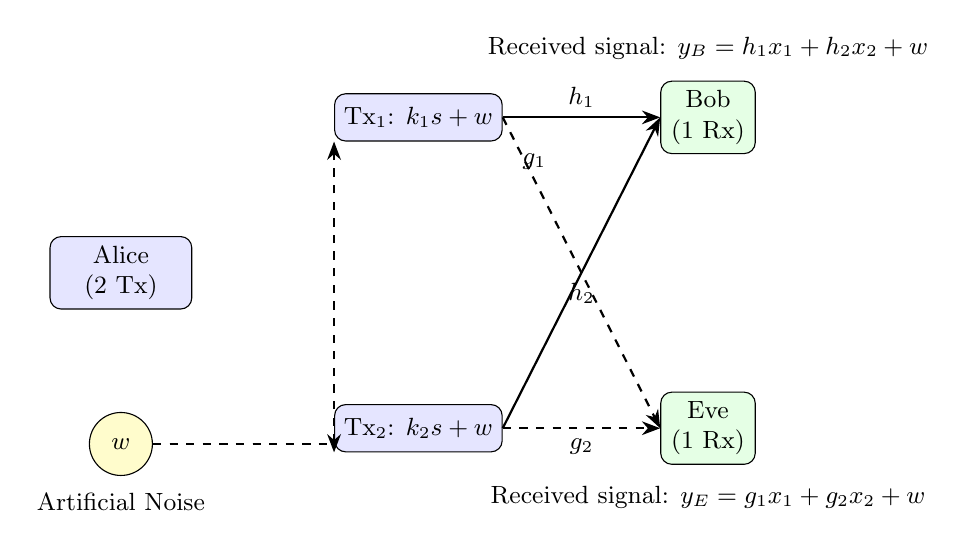
\begin{tikzpicture}[
    node distance=1cm and 1cm,
    every node/.style={font=\small},
    tx/.style={rectangle, draw, rounded corners, fill=blue!10, align=center, minimum width=1.8cm, minimum height=0.6cm},
    rx/.style={rectangle, draw, rounded corners, fill=green!10, align=center, minimum width=1.2cm, minimum height=0.6cm},
    sum/.style={circle, draw, fill=yellow!20, minimum size=8mm, inner sep=0pt , align = center},
    line/.style={-Stealth, thick}
]

% Nodes for Alice
\node[tx] (alice) {Alice\\(2 Tx)};
\node[tx, above right=1.2cm and 1.8cm of alice] (tx1) {Tx$_1$: $k_1s+ w$};
\node[tx, below right=1.2cm and 1.8cm of alice] (tx2) {Tx$_2$: $k_2s + w$};

% Bob and Eve receivers
\node[rx, right=2cm of tx1] (bob) {Bob\\(1 Rx)};
\node[rx, right=2cm of tx2] (eve) {Eve\\(1 Rx)};

% Channel labels for Bob
\draw[line] (tx1.east) -- node[above] {$h_1$} (bob.west);
\draw[line] (tx2.east) -- node[below] {$h_2$} (bob.west);

% Clean dashed lines for Eve (avoiding intersections)
\draw[line, dashed] (tx1.east) -- node[pos=0.2, above] {$g_1$} (eve.west); % <-- direct line for g1

\draw[line, dashed] (tx2.east) -- node[pos=0.5, below] {$g_2$} (eve.west);

% Labels for received signals
\node[above=0.15cm of bob] {Received signal: $y_B = h_1x_1 + h_2x_2 + w$};
\node[below=0.15cm of eve] {Received signal: $y_E = g_1x_1 + g_2x_2 + w$};

% Artificial noise source
\node[sum, below=1.3cm of alice] (noise) {$w$};
\draw[line, dashed] (noise) -| (tx1.south west);
\draw[line, dashed] (noise) -| (tx2.south west);
\node[below=0.1cm of noise] {Artificial Noise};

\end{tikzpicture}
\end{tcolorbox}

% \subsubsection{Channel State Information Exploitation}

% \begin{tcolorbox}[colback=white,colframe=black,boxrule=2pt,arc=0.5mm,title=\textcolor{accentyellow}{\textbf{CSI-Based Security Strategies}}]
% \color{black}
% \begin{enumerate}[leftmargin=*,itemsep=0.15cm]
%   \item \textbf{Channel Measurement:} Alice and Bob perform channel sounding with training sequences
%   \item \textbf{CSI Feedback:} Bob reports channel quality metrics to Alice via secure reverse link
%   \item \textbf{Reciprocity Exploitation:} TDD mode leverages Alice-Bob channel reciprocity (Bob's CSI for Alice)
%   \item \textbf{Quantization and Feedback:} Bob quantizes CSI to $Q$ bits, exploiting quantization noise
%   \item \textbf{Secrecy Beamforming:} Alice constructs transmit precoder based on Bob's reported CSI
%   \item \textbf{Artificial Noise Design:} Precoder creates harmful interference aligned with Eve's null space
% \end{enumerate}
% \end{tcolorbox}

% \subsection{Performance Metrics for Security}

% \begin{tcolorbox}[colback=white,colframe=black,boxrule=2pt,arc=0.5mm,title=\textcolor{accentyellow}{\textbf{Key Security Metrics}}]
% \color{black}
% \begin{description}[leftmargin=2.5cm,font=\textbf]
%   \item [Secrecy Capacity:] $C_s = [I(X;Y) - I(X;Z)]^+$ bits per channel use
%   \item [Information Leakage:] Mutual information $I(X;Z)$ available to eavesdropper
%   \item [Secure Outage Probability:] Probability that $C_s < R_s$ (secrecy rate requirement)
%   \item [Perfect Secrecy Rate:] Maximum rate guaranteeing zero information leakage
%   \item [Eve's Equivocation Rate:] Entropy of plaintext given Eve's observations
% \end{description}
% \end{tcolorbox}

% \subsubsection{Experimental Validation}

% \begin{tcolorbox}[colback=white,colframe=black,boxrule=2pt,arc=0.5mm]
% \color{black}
% \textbf{Validation Procedure:}
% \begin{enumerate}[leftmargin=*,itemsep=0.15cm]
%   \item Establish three synchronized USRP nodes in controlled RF environment
%   \item Implement beamforming transmissions with artificial noise injection
%   \item Measure Bob's and Eve's received SNR at synchronized time instants
%   \item Compute achievable rates for both receivers using Shannon capacity
%   \item Log channel impulse responses for post-processing analysis
%   \item Evaluate decoding success rates at various secrecy margin targets
%   \item Quantify information leakage through mutual information estimation
% \end{enumerate}
% \end{tcolorbox}

\section{Implementation Process Flow}

\begin{tcolorbox}[
  colback=gray!5,
  colframe=black!80,
  title=\textbf{MATLAB-Based Simulation Framework},
  fonttitle=\bfseries,
  sharp corners
]
The initial part of the work focused on building a complete Physical Layer Security (PLS) simulation environment in \textbf{MATLAB}. This included:
\begin{itemize}
    \item Modeling the Alice–Bob–Eve system under wireless fading channels.
    \item Implementing OFDM modulation, demodulation, and equalization.
    \item Simulating independent channels for both Bob and Eve.
    \item Verifying theoretical concepts, including:
    \begin{itemize}
        \item Accurate channel estimation and equalization
        \item Secure data transmission mechanisms
        \item Performance comparison between Bob and Eve under identical conditions
    \end{itemize}
\end{itemize}

These simulations provided a solid theoretical baseline before transitioning to real hardware experiments.
\end{tcolorbox}


\section{Exploration of GNU Radio}

\begin{tcolorbox}[
  colback=blue!3,
  colframe=blue!80!black,
  title=\textbf{Real-Time Signal Processing with GNU Radio},
  fonttitle=\bfseries,
  sharp corners
]
We next explored \textbf{GNU Radio} for real-time baseband processing and integration with USRP devices.  
The objective was to implement dual-antenna transmission from Alice and simultaneous reception at Bob and Eve.

\subsection*{Work Undertaken}
\begin{itemize}
    \item Designed OFDM-based flowgraphs using built-in and custom blocks.
    \item Experimented with:
    \begin{itemize}
        \item OFDM modulation/demodulation blocks
        \item Tag-based frame synchronization
        \item Channel estimation and equalizer modules
    \end{itemize}
    \item Evaluated multi-USRP synchronization and data transport.
\end{itemize}

\subsection*{Challenges Encountered}
\begin{itemize}
    \item Timing and synchronization complexities in GNU Radio.
    \item Tag-management overhead for multi-antenna, multi-frame transmission.
    \item Debugging real-time data flow between multiple USRPs proved difficult.
\end{itemize}
\end{tcolorbox}


\section{Experimental Setup with USRPs}

\begin{tcolorbox}[
  colback=green!4,
  colframe=green!45!black,
  title=\textbf{Hardware Implementation Using USRPs},
  fonttitle=\bfseries,
  sharp corners
]
The hardware configuration included:
\begin{itemize}
    \item \textbf{Two USRPs at Alice} for Tx1 and Tx2.
    \item \textbf{One USRP at Bob} (legitimate receiver).
    \item \textbf{One USRP at Eve} (eavesdropper).
\end{itemize}

\subsection*{Procedure}
\begin{itemize}
    \item Both transmit chains at Alice were synchronized for dual transmission.
    \item Distinct OFDM frames were sent simultaneously from Tx1 and Tx2.
    \item Bob received the combined signals and processed them in real-time using MATLAB.
\end{itemize}
\end{tcolorbox}


\section{Achievements}

\begin{tcolorbox}[
  colback=yellow!6,
  colframe=orange!85!black,
  title=\textbf{Key Achievements So Far},
  fonttitle=\bfseries,
  sharp corners
]
Major accomplishments include:
\begin{itemize}
    \item Achieved \textbf{simultaneous dual-antenna transmission} from Alice.
    \item Bob successfully \textbf{received and decoded} both data streams.
    \item Implemented a complete \textbf{channel equalization} pipeline at the receiver.
    \item Extracted and visualized the individual channel responses:
    \begin{itemize}
        \item Tx1 $\rightarrow$ Bob
        \item Tx2 $\rightarrow$ Bob
    \end{itemize}
    \item Verified synchronization across all USRPs and validated channel estimation accuracy.
\end{itemize}
\end{tcolorbox}


\section{Organisation}

\subsection{Common Framework}

All four projects share a unified signal processing framework implemented across multiple components:

\begin{tcolorbox}[colback=white,colframe=black,boxrule=2pt,arc=0.5mm,title=\textcolor{white}{\textbf{Cross-Project Common Elements}}]
\color{black}
\begin{itemize}[leftmargin=*,itemsep=0.2cm]
  \item \textbf{Modulation Base:} OFDM with configurable subcarrier count and modulation schemes
  \item \textbf{Synchronization:} Timing offset detection via preamble correlation
  \item \textbf{Channel Estimation:} Least-squares or MMSE channel estimation on training symbols
  \item \textbf{Equalization:} Single-tap frequency-domain equalization per subcarrier
  \item \textbf{Coding:} Convolutional codes with Viterbi decoding
  \item \textbf{Logging Framework:} Centralized data acquisition for performance analysis
\end{itemize}
\end{tcolorbox}

\subsection{File Organization and Data Flow}

The implementation organizes code across project folders with specialized modules:

\begin{tcolorbox}[colback=white,colframe=black,boxrule=2pt,arc=0.5mm,title=\textcolor{white}{\textbf{Directory Structure}}]
\color{black}
\begin{description}[leftmargin=3cm,font=\texttt\small,labelwidth=3cm]
  \item[Global\_Parameters\_PLS.m] : Master configuration file (center frequency, gains, packet structure)
  \item[OFDM\_TX\_X.m] : OFDM transmitter implementation for node X (Alice/Bob/Eve)
  \item[OFDM\_RX\_X.m] : OFDM receiver with equalization and synchronization
  \item[Hardware\_TX\_X.m] : USRP/Pluto hardware interface (DAC buffering, gain control)
  \item[Hardware\_RX\_X.m] : Hardware receiver interface (ADC streaming, data logging)
  \item[corr\_code.m] : Preamble correlation for timing synchronization
  \item[oversamp.m] : Oversampling and pulse shaping filters
  \item[setstate0\_TX/RX.m] : USRP initialization and state reset
\end{description}
\end{tcolorbox}


\section{Development Methodology and Lessons Learned}

\subsection{Iterative Development Process}

\begin{tcolorbox}[colback=white,colframe=black,boxrule=2pt,arc=0.5mm]
\color{black}
\textbf{Project Development Cycle:}
\begin{enumerate}[leftmargin=*,itemsep=0.15cm]
  \item \textbf{Simulation:} Algorithm development and validation in MATLAB/Simulink
  \item \textbf{Hardware Integration:} Porting to USRP drivers and real-time constraints
  \item \textbf{Bench Testing:} Validation with test signals in RF-isolated environment
  \item \textbf{Over-the-Air Testing:} Evaluation in actual propagation conditions
  \item \textbf{Performance Analysis:} Statistical evaluation of measured data
  \item \textbf{Optimization:} Parameter tuning based on empirical results
\end{enumerate}
\end{tcolorbox}

\subsection{Key Technical Challenges and Solutions}
\begin{tcolorbox}[colback=white,colframe=black,boxrule=2pt,arc=0.5mm,title=\textcolor{accentyellow}{\textbf{Key Security Metrics}}]
\color{black}
\begin{description}[leftmargin=2.5cm,font=\textbf]
  \item [Timing Misalignment:] Implemented coarse/fine synchronization with preamble correlation and feedback loops
  \item [Frequency Offsets:] Developed pilot-based frequency correction with loop bandwidth optimization
  \item [Channel Fading:] Applied equalization
  \item [Cross-Device Sync:] Distributed reference clocks and GPS time tagging
  \item [Real-Time Performance:] Optimized code for USRP's real-time 
\end{description}
\end{tcolorbox}







\chapter{Cross-Platform Comms}
\ChapterCredits{
    Dhanush V Nayak
    Kaustubh Khachane
}
\section{The Big Picture}
We are building a security system where Alice (USRP B210) sends a secret message using two antennas, and Bob (Adalm Pluto) tries to receive it using one antenna.

\begin{conceptbox}{The Main Challenge}
The USRP and the Pluto are like two people who speak different dialects and hence different way of handling things. Just to list :
\begin{itemize}
    \item \textbf{USRP}Our Alice has to send and receive data and also do channel processing.
    \item \textbf{Pluto} Bob has to just receive and decode the data.
\end{itemize}
To make them understand each other and make good use of the hardware, we must force them to speak at exactly the same speed (3 MHz).
\end{conceptbox}

\section{Step 1: The Hardware Setup}

We use "Objects" in MATLAB to control the hardware. Here is how we configured them in \texttt{TX\_dual\_pluto.m} and \texttt{Hardware\_RX\_Bob.m}.

\vspace{0.5cm}

\begin{alicebox}{Alice: The Transmitter}
Alice is the "Master" of the transmission. She sends two signals at once.

\begin{itemize}
    \item \textbf{Device:} USRP B210
    \item \textbf{Goal:} Send separate streams on Antenna 1 and Antenna 2.
    \item \textbf{The Trick:} We use \textbf{Interpolation} to slow down the internal clock to a speed the Pluto can handle.
\end{itemize}

\textbf{Key Settings:}
\begin{enumerate}
    \item \texttt{MasterClockRate = 30 MHz} (Internal Heartbeat)
    \item \texttt{InterpolationFactor = 10} (Slow down by 10x)
    \item \textbf{Resulting Speed:} $30 \text{ MHz} / 10 = \mathbf{3 \text{ MHz}}$
    \item \texttt{ChannelMapping = [1 2]} (Use both antennas)
\end{enumerate}
\end{alicebox}

\vspace{0.5cm}

\begin{bobbox}{Bob: The Receiver}
Bob is the listener. He uses a cheaper radio, so we have to tell him exactly what to listen for.

\begin{itemize}
    \item \textbf{Device:} Adalm Pluto (PlutoSDR)
    \item \textbf{Goal:} Listen to Alice and separate her two signals.
    \item \textbf{The Trick:} We force the Pluto's "Baseband Rate" to match Alice exactly.
\end{itemize}

\textbf{Key Settings:}
\begin{enumerate}
    \item \texttt{BasebandSampleRate = 3 MHz} (Must match Alice!)
    \item \texttt{CenterFrequency = 800 MHz} (Must match Alice)
    \item \texttt{Gain = 60 dB} (High gain because Pluto is less sensitive)
\end{enumerate}
\end{bobbox}


\section{Step 2: How Bob Finds the Message}

The air is full of noise. Bob needs a way to know "Hey, a message is starting now!"

\subsection*{The Packet Detection}
Alice sends a special pattern called a Preamble at the start of every message. This acts like a message to capture the data.

\begin{conceptbox}{Schmidl-Cox Algorithm (Simple Explanation)}
\begin{enumerate}
    \item Alice sends a short pattern: \texttt{[A, A, A, A]}.
    \item Bob constantly compares the signal he just received with the signal he received a split second ago.
    \item If \textbf{Current Signal} looks exactly like \textbf{Past Signal}, Bob knows it's the repeating preamble.
    \item \textbf{Math:} We calculate a score $M(n)$. When $M(n) > 0.6$, we trigger the recording.
\end{enumerate}
\end{conceptbox}

\section{Step 3: Separating the Two Antennas}

This is the most critical part of Physical Layer Security. Bob has only \textbf{one ear} (antenna), but Alice is speaking with \textbf{two mouths} (Tx1 and Tx2). How does he know who said what?

\subsection*{The "Pilot" Solution}
We use \textbf{Orthogonal Pilots}.Please refer to the codes in the same folder for more detail.

\begin{center}
\begin{tabular}{|c|c|c|}
\hline
\rowcolor{gray!20} \textbf{Frequency Key} & \textbf{Tx1 Action} & \textbf{Tx2 Action} \\
\hline
Key \#16 & \textbf{Signal1} & Silent(Null) \\
\hline
Key \#18 & Silent & \textbf{Signal2} \\
\hline
Key \#24 & \textbf{Signal1} & Silent \\
\hline
Key \#26 & Silent & \textbf{Signal2} \\
\hline
\end{tabular}
\end{center}

\begin{enumerate}
    \item Bob listens to Key \#16. He hears a sound. Since he knows Tx2 is silent there, \textbf{that sound must describe Tx1's channel.}
    \item Bob listens to Key \#18. He hears a sound. Since he knows Tx1 is silent there, \textbf{that sound must describe Tx2's channel.}
\end{enumerate}

\section{Summary: The Code Logic}

Here is the flow of \texttt{OFDM\_RX\_Bob.m} in plain English:

\begin{tcolorbox}[colback=yellow!10, colframe=orange!80!black, title=The Receiver Logic Chain]
\begin{enumerate}
    \item \textbf{Wait} for the trigger signal ($M_n > 0.6$).
    \item \textbf{Cut} the signal into a "Frame" (480 samples).
    \item \textbf{Correct} the frequency (Pluto and USRP clocks are slightly different, so we rotate the signal back).
    \item \textbf{Extract} the Pilot Keys (indices 16, 18, 24, etc.).
    \item \textbf{Calculate} Channel 1 from the Tx1 keys.
    \item \textbf{Calculate} Channel 2 from the Tx2 keys.
    \item \textbf{Decode} the secret message using these channel estimates.
\end{enumerate}
\end{tcolorbox}



\twocolumn
\chapter{USRP X310 in MATLAB}
\ChapterCredits{
    Prabhat Kukunuri,
    Varun Shakunaveti,
    Anantha Krishnan
}

\section{Overview}

The Universal Software Radio Peripheral (USRP) X310, developed by Ettus Research,
is a reconfigurable software-defined radio (SDR) platform designed for real-time
signal processing and high-bandwidth wireless communication experimentation. Its
FPGA-based design, support for wideband radios, and compatibility with
open-source tools make it especially suitable for cognitive radio, MIMO systems,
and radar research.

By integrating flexible RF modules, the system can cover a wide frequency range
and adapt to diverse wireless standards. The X310 architecture enables
high-speed streaming through 10~Gigabit Ethernet, supporting low-latency
data transfer for demanding research applications.

\section{Hardware Architecture}

The core of the X310 is the Xilinx Kintex-7 FPGA, which performs computationally
intensive baseband operations such as filtering, modulation, and timing
synchronization. The system supports dual RF daughterboards with independent
transmit and receive chains.

Key hardware components include:
\begin{itemize}
    \item Xilinx Kintex-7 (XC7K410T) FPGA
    \item Dual DACs (16-bit) and dual ADCs (14-bit)
    \item 10~Gigabit Ethernet and PCIe~x4 host interfaces
    \item GPSDO / external reference timing support
\end{itemize}

\section{Software Stack and UHD Integration}

The USRP Hardware Driver (UHD) provides the primary software interface to the
USRP X310. UHD exposes a unified API for configuration, streaming, tuning, gain
control, and synchronization, and integrates with several higher-level tools:
\begin{itemize}
    \item GNU Radio
    \item MATLAB/Simulink
    \item C/C++ and Python-based applications
\end{itemize}

In the experiments described in this chapter, UHD is accessed primarily through
MATLAB support packages, which internally rely on UHD for device discovery,
streaming, and control.

\section{Host and Network Setup}

This section describes the practical steps required to power, network, and
probe the USRP X310 from a host machine.

\subsection*{Power and Basic Connectivity}

\begin{enumerate}
    \item Connect the power supply to the USRP X310 and then to the AC mains.
    \item Switch on the USRP using the front-panel power control (if available).
    Status LEDs indicate power and initialization state.
    \item On the host PC, configure the Ethernet interface to communicate with
    the USRP via UHD. Select the Ethernet interface connected to the USRP and
    change the IP assignment mode to \textbf{Manual} (or \textbf{Static}) with
    the following IPv4 settings:
    \begin{itemize}
        \item IPv4 Address: \texttt{192.168.10.1}
        \item Subnet Mask: \texttt{255.255.255.0}
        \item Default Gateway: (leave blank or set to \texttt{0.0.0.0})
    \end{itemize}
    After applying these settings, the host and the USRP reside on the same
    subnet. Basic connectivity can be verified by issuing a \texttt{ping}
    command to the USRP’s default IP address:
    \begin{lstlisting}
ping 192.168.10.2
    \end{lstlisting}
    A representative successful output is:
    {\footnotesize
    \begin{lstlisting}
Pinging 192.168.10.2 with 32 bytes of data:
Reply from 192.168.10.2: bytes=32 time=1ms TTL=32
Reply from 192.168.10.2: bytes=32 time=3ms TTL=32
Reply from 192.168.10.2: bytes=32 time=3ms TTL=32
Reply from 192.168.10.2: bytes=32 time=3ms TTL=32

Ping statistics for 192.168.10.2:
    Packets: Sent = 4, Received = 4, Lost = 0 (0% loss),
Approximate round trip times in milli-seconds:
    Minimum = 1ms, Maximum = 3ms, Average = 2ms
    \end{lstlisting}
    }
    The absence of packet loss confirms that the network configuration is
    correct and the device is reachable.
    \item Use the UHD probing utility to confirm that the device and
    daughterboards are correctly recognized:
    \begin{lstlisting}
uhd_usrp_probe --args="addr=192.168.10.2"
    \end{lstlisting}
    This command reports information such as device type, serial number,
    installed daughterboards, clock sources, and available channels.
\end{enumerate}

\subsection*{Firmware and FPGA Image Update}

For reliable operation, the USRP X310 should run a firmware and FPGA image
version compatible with the installed UHD release. If a version mismatch is
detected, UHD utilities can be used to update the images:

\begin{enumerate}
    \item Install the appropriate UHD version on the host PC.
    \item Download or locate the device images (firmware and FPGA bitstreams)
    distributed with UHD.
    \item Use the image loading utility to program the X310:
    {\footnotesize
    \begin{lstlisting}
uhd_image_loader --args="type=x300,addr=192.168.10.2"
    \end{lstlisting}
    }
    \item After the image is successfully written, power-cycle the USRP X310.
    \item Re-run \texttt{uhd\_usrp\_probe} to confirm that the device now
    reports the expected image versions.
\end{enumerate}

\section{MATLAB Integration}

This section focuses on the MATLAB software requirements and the specific radio
interfaces used in the experiments.

\subsection*{Required Toolboxes and Support Packages}

To interface USRP radios such as the X310 from MATLAB and conduct SDR
experiments, the following components are required:
\begin{itemize}
  \item MATLAB (base environment)
  \item \textbf{Communications Toolbox} --- for modulation/demodulation, filters,
        and baseband operations
  \item \textbf{Signal Processing Toolbox} --- for DSP operations, filtering,
        FFT, and spectral analysis
  \item \textbf{DSP System Toolbox} --- for advanced DSP functions, streaming,
        block-based systems, and real-time data handling
  \item \textbf{Wireless Testbench Support Package for NI USRP Radios} ---
        for X-series (X300 / X310 / X410) or N3xx-series USRPs
\end{itemize}

\subsection*{sdruTransmitter and sdruReceiver Interface}

The \texttt{sdruTransmitter} and \texttt{sdruReceiver} System objects in MATLAB
provide a legacy interface to USRP hardware for wireless baseband transmission
and reception. These objects allow streaming of IQ sample frames between MATLAB
and the USRP radio using the UHD driver.

\subsubsection*{Overview of Transmitter and Receiver Objects}

\begin{itemize}
    \item \textbf{\texttt{sdruTransmitter}}: used to send complex baseband
    samples from MATLAB to the USRP RF front-end. Key parameters include center
    frequency, gain, interpolation factor, and channel mapping.
    
    \item \textbf{\texttt{sdruReceiver}}: used to capture IQ samples from the
    USRP into MATLAB for processing. Important properties include center
    frequency, gain, decimation factor, sample rate, and frame size.
\end{itemize}

Once configured, both objects operate using the \texttt{step()} function inside
a streaming loop. The loop ensures continuous transmission or reception of
frames until manually stopped.

\subsubsection*{Example: Transmit and Receive IQ Frames}

The following simple example illustrates the creation of transmitter and
receiver objects, followed by a \texttt{for}-loop for real-time transmission and
reception of signals:

\begin{lstlisting}[language=MATLAB]
% Create transmitter and receiver objects
tx = sdruTransmitter('192.168.10.2', ...
    'CenterFrequency', 2.4e9, ...
    'Gain', 20);

rx = sdruReceiver('192.168.10.2', ...
    'CenterFrequency', 2.4e9, ...
    'Gain', 15, ...
    'SamplesPerFrame', 1024);

% Generate a baseband test signal
txSignal = exp(1j*2*pi*0.01*(0:1023)).';

% Streaming loop
for k = 1:100
    % Transmit a frame
    step(tx, txSignal);

    % Receive a frame
    rxSignal = step(rx);
    
    % Simple processing (e.g., display received energy)
    disp(mean(abs(rxSignal).^2));
end

% Release radio objects
release(tx);
release(rx);
\end{lstlisting}

The transmit object must be called continuously inside the streaming loop;
otherwise, the USRP will run out of samples and the transmission will stop due
to a buffer underflow condition.

In some cases, especially after power cycling the USRP or restarting MATLAB, it
is necessary to reload the FPGA image on the USRP X310 before streaming can
begin. This ensures that the firmware and image versions are synchronized with
the installed UHD and MATLAB support package. The following command can be used
to reconfigure the image on the device before running the transmit and
receive operations:

% {\scriptsize
\begin{lstlisting}
status=sdruload('Device','X310','IPAddress','192.168.10.2');
\end{lstlisting}
% }
A successful execution of this command confirms that the X310 is correctly
programmed and ready for baseband transmission and reception.

\subsection*{Wireless Testbench sdrtx / sdrrx Interface}

In addition to the legacy \texttt{sdru} interface, newer MATLAB workflows rely
on the Wireless Testbench \texttt{sdrtx} and \texttt{sdrrx} System objects. These
objects integrate directly with the support package for NI USRP radios and
provide convenient functions such as \texttt{transmitRepeat}.

Before executing scripts that use these objects, the USRP X310 must first be
initialized as part of the Wireless Testbench Support Package installation.
During this process, the Radio Setup wizard is launched from
\texttt{Add-Ons}~$\rightarrow$~\texttt{Manage Add-Ons}~$\rightarrow$~\texttt{Hardware Setup},
where the user selects the NI USRP hardware and configures the connection
settings. The wizard automatically detects the X310 on the network, verifies
IP connectivity, and updates the FPGA image and firmware if necessary. After
this initialization, MATLAB transmitter and receiver System objects can
communicate with the USRP using the assigned device identifier or IP address.

\section{Baseband Transmitter and Receiver Design}

In the proposed setup, the USRP X310 is controlled from MATLAB and operates as
a baseband transmitter--receiver pair. A complex baseband frame is first
generated in MATLAB and then uploaded to the radio. The transmitter is
configured to continuously retransmit this buffer, while the receiver runs in a
loop and acquires incoming IQ samples for further processing.

\subsection*{Baseband Transmitter}

The baseband transmitter generates a complex-valued IQ sequence, which may
represent a test tone, a modulated symbol stream, or a training sequence. This
frame is sent once to the USRP using a transmit object. Instead of calling the
transmitter inside a loop, the hardware is instructed to repeat the same frame
indefinitely, so the transmit operation runs in the background on the USRP.

\subsection*{Baseband Receiver}

The baseband receiver is implemented as a corresponding receive object in
MATLAB. The receiver is executed inside a \texttt{for}-loop, where a new frame
of IQ samples is captured from the USRP in each iteration. These received
frames can then be used for spectrum analysis, synchronization, correlation
with a known preamble, or bit-error rate (BER) computation. In this way, the
transmitter operates continuously, while the receiver processes a stream of
frames in real time.

\subsection*{Baseband Transmitter and Receiver Example in MATLAB}

% {\scriptsize
\begin{lstlisting}[language=MATLAB]
%% Baseband Transmitter and Receiver with USRP X310
% Assumes:
% - Wireless Testbench / USRP support package installed
% - USRP X310 reachable at the given device name or IP

fc       = 2.4e9;     % Center frequency
fs       = 1e6;       % Sample rate
txGain   = 20;        % Transmit gain (dB)
rxGain   = 15;        % Receive gain (dB)
frameLen = 2048;      % Samples per frame
numFrames = 200;      % Number of frames to receive

%% Create Transmitter Object
tx = sdrtx('USRP X310', ...
    'CenterFrequency', fc, ...
    'Gain',           txGain, ...
    'BasebandSampleRate', fs);

%% Create Receiver Object
rx = sdrrx('USRP X310', ...
    'CenterFrequency',     fc, ...
    'Gain',                rxGain, ...
    'BasebandSampleRate',  fs, ...
    'SamplesPerFrame',     frameLen, ...
    'OutputDataType',     'double');

%% Generate Baseband Transmit Frame (example: complex tone)
n       = (0:frameLen-1).';
txFrame = exp(1j*2*pi*0.01*n);   % simple complex exponential
txFrame = txFrame ./ max(abs(txFrame));  % normalize

%% Start Continuous Transmission on Hardware
transmitRepeat(tx, txFrame);
disp('Tx is continuously replaying the baseband frame...');

%% Continuous Reception Loop
for k = 1:numFrames
    rxSig = rx();
    
    % compute and display average received power
    rxPower = mean(abs(rxSig).^2);
    fprintf('Frame %d: Rx power = %.3f\n', k, rxPower);
end

%% Stop Transmission and Release Hardware
release(tx);
release(rx);
\end{lstlisting}

\section{Difficulties Faced}

During the implementation of the baseband transmitter and receiver using the
USRP X310 and MATLAB, several practical difficulties were encountered. These
issues affected the signal levels, workflow efficiency, and flexibility of the
software environment.

\subsection*{Low Transmit and Receive Power}

One of the main issues observed was that the received and transmitted signal
powers were significantly lower than expected. Even after successful
configuration of the center frequency and sample rate, the effective RF power
at the receiver side remained low. This was primarily attributed to
insufficient gain settings on the transmitter and receiver chains. As a result,
the received signal-to-noise ratio (SNR) was degraded, making it more difficult
to reliably observe and process the transmitted waveform without further
amplification or gain adjustment.

\subsection*{Frequent FPGA Image Reconfiguration}

Another notable difficulty was the frequent need to re-burn or reload the FPGA
image on the USRP X310 from within MATLAB. In order to switch between different
configurations or dependencies (e.g., different MATLAB support packages, UHD
versions, or experimental setups), the image often had to be reconfigured using
commands such as:
% {\footnotesize
\begin{lstlisting}
status = sdruload('Device','X310','IPAddress','192.168.10.2');
\end{lstlisting}
% }
This repeated image loading added considerable overhead to the workflow and
increased setup time before each experiment, especially when the device was
power-cycled or when changing between multiple test scenarios.

\subsection*{Scripting Software Limitations}

Another major difficulty encountered was related to the MATLAB scripting
environment itself. Since MATLAB does not natively support multithreading for
System object execution, the entire transmit--receive chain runs as a single
threaded process. This significantly limits real-time performance when handling
high-rate streaming or processing-intensive algorithms. As a result, the CPU
workload frequently became a bottleneck, restricting the maximum achievable
sampling rates and the responsiveness of the system.

Additionally, the availability of detailed documentation and example resources
specifically for the USRP X310 in MATLAB was limited. Most online support and
open-source code repositories were focused on GNU Radio or UHD C++ workflows,
making it difficult to troubleshoot MATLAB-specific integration issues. This
lack of reference material and debugging guidance contributed to increased
development time and experimentation overhead.

% \chapter{Beamforming}
\section{Introducing Beamforming}
In modern RADAR and communication systems, \textbf{beamforming} is a key technique used to direct the reception or transmission of signals in specific spatial directions. The ability to estimate the \textbf{Angle of Arrival (AoA)} of a received signal enables systems to locate and track active sources or targets.

We now present the implementation of \textbf{monopulse beamforming} using an \textbf{ADALM-Pluto Software Defined Radio (SDR)}. The system transmits a known reference tone, receives it through a two-element antenna array, and estimates the AoA of an active target based on the \textbf{phase difference} between received signals.

\section{Digital Beamforming}
\subsection{Concept Overview}
\textbf{Digital Beamforming (DBF)} is a signal processing technique in which the signals received by multiple antenna elements are digitized and combined in the \textit{digital domain} using complex weighting coefficients.  
By adjusting these weights, the system can electronically steer the main beam toward a desired direction or place nulls toward unwanted sources — all without physically moving the antennas.

Unlike analog beamforming, which relies on hardware-based phase shifters and combiners, digital beamforming performs all spatial filtering and steering in software, offering high flexibility, adaptability, and precision.

\subsection{Mathematical Model}
Consider an array of $N$ antenna elements receiving a narrowband signal $s(t)$ arriving from direction $\theta$.  
The received signal vector can be expressed as:
\begin{equation}
    \mathbf{x}(t) = s(t)\mathbf{a}(\theta) + \mathbf{n}(t)
\end{equation}
where:
\begin{itemize}
    \item $\mathbf{a}(\theta)$ is the \textit{steering vector}, which represents the phase progression across antennas for a signal from direction $\theta$,
    \item $\mathbf{n}(t)$ is the noise vector.
\end{itemize}

For two receivers with inter-element spacing $d$, the steering vector is given by:
\begin{equation}
    \mathbf{a}(\theta) =
    \begin{bmatrix}
    1 \\
    e^{-j\frac{2\pi d}{\lambda}\sin(\theta)} \\
    \end{bmatrix}
\end{equation}

The beamformer output is obtained by applying a complex weight vector $\mathbf{w}$:
\begin{equation}
    y(t) = \mathbf{w}^H \mathbf{x}(t)
\end{equation}

\subsection{Beam Steering}
To steer the beam toward a desired angle $\theta_0$, the weights are typically chosen proportional to the steering vector:
\begin{equation}
    \mathbf{w} = \mathbf{a}(\theta_0)
\end{equation}
This choice ensures that signals arriving from $\theta_0$ add constructively across the array, maximizing gain in that direction while causing destructive interference in the other directions.

\section{Theory}
\subsection{Angle of Arrival Calculation}
If two antennas receive a plane wave at slightly different phases due to path delay, the phase difference $\Delta \phi$ can be used to compute the angle of arrival $\theta$:

\begin{equation}
    \Delta \phi=\frac{2\pi d\sin{\theta}}{\lambda}
\end{equation}

\begin{itemize}
    \item $f$ — carrier frequency (Hz),
    \item $d$ — antenna spacing (m),
    \item $\Delta \phi$ — measured phase difference (radians).
\end{itemize}

Hence:
\begin{equation}
    \theta = \arcsin\left(\frac{c \, \Delta \phi}{2\pi f d}\right)
\end{equation}

Here we consider the received signals to be parallel rather than circular, hinting that we need to place the active transmitter very far away from the receiver antennas.\\

We place the received antennas at a distance of $\frac{\lambda}{2}$ of the carrier frequency to avoid antenna interference. 

\subsection{Monopulse Technique}
Monopulse beamforming combines two signals to form sum and difference channels:

\begin{align}
    \Sigma &= R_1 + R_2 \\
    \Delta &= R_1 - R_2
\end{align}

The \textbf{sum channel} represents the total received power, while the \textbf{difference channel} captures the angular error. The correlation between $\Sigma$ and $\Delta$ 
provides the direction to steer the antenna array.

When the sum and the delta signals are represented in complex version and then we take correlation at then the delay is 0, it becomes inner product on further solving it turns to be a $\sin{(\theta-\phi)}$ as we use this for tracking we can make an assumption that is the difference is very small and small angle approximation is used.
\begin{align*}
    \theta&:\text{The original received phase difference}\\
    \phi&:\text{The sweeping angle}
\end{align*}
The sign of the correlation tells us which direction to steer the sweep angle. When the beam is aligned with the target, $\Delta \approx 0$, indicating zero angle error.

\subsection{Proof - Frequency domain correlation}

Let the observed signals at the two receivers be
\[
x_0(t) = A e^{j2\pi f_0 t}
\]
\[
x_1(t) = A e^{j2\pi f_0 t} e^{j\phi}
\]
where $A$ is amplitude, $f_0$ is the signal frequency, and $\phi$ is the phase offset due to the signal's direction of arrival (DOA).

Apply a steering phase $\phi_{\text{delay}}$ to $x_1(t)$:
\[
\Sigma(t) = x_0(t) + x_1(t) e^{j\phi_{\text{delay}}} = A e^{j2\pi f_0 t}[1 + e^{j\epsilon}]
\]
\[
\Delta(t) = x_0(t) - x_1(t) e^{j\phi_{\text{delay}}} = A e^{j2\pi f_0 t}[1 - e^{j\epsilon}]
\]
\[\epsilon = \phi - \phi_{\text{delay}}\]
Perform a Fourier Transform of these signals:
\begin{align*}
S = \Sigma(f_0) &= A[1 + e^{j\epsilon}] \\
D = \Delta(f_0) &= A[1 - e^{j\epsilon}]
\end{align*}

Compute the frequency domain correlation at the tone:
\begin{align*}
\mathrm{Corr} &= S^* D = [A(1 + e^{j\epsilon})]^* \cdot [A(1 - e^{j\epsilon})] \\
&= A^2 (1 + e^{-j\epsilon})(1 - e^{j\epsilon}) \\
&= A^2 [1 - e^{j\epsilon} + e^{-j\epsilon} - e^{-j\epsilon}e^{j\epsilon}] \\
&= A^2 [1 - e^{j\epsilon} + e^{-j\epsilon} - 1] \\
&= A^2 [ -e^{j\epsilon} + e^{-j\epsilon} ] \\
&= -A^2 [ e^{j\epsilon} - e^{-j\epsilon} ] \\
&= -A^2 [2j\sin\epsilon ] \\
&= -2jA^2 \sin(\epsilon)
\end{align*}

Thus, the correlation is purely imaginary, and the sign of its imaginary part reveals which direction to adjust the steering phase:
- If $\sin(\epsilon) > 0$: $\mathrm{Corr}$ phase is $-90^\circ$ (steer phase down)
- If $\sin(\epsilon) < 0$: $\mathrm{Corr}$ phase is $+90^\circ$ (steer phase up)
.

\subsection{Parseval's Theorem}
Parseval's theorem states that the total energy of a signal is preserved between time and frequency domains:
\[
\sum_{n} x[n] y^*[n] = \frac{1}{N}\sum_{k} X[k] Y^*[k]
\]
where $x[n]$ and $y[n]$ are discrete signals and $X[k], Y[k]$ are their DFTs. The reason i have mentioned this is because we can do the exact same process with the time domain signals (we get the same function as above, although scaled but we only care about the sign) for steering the array.

\section{Algorithm Description}
\subsection{Step 1: Signal Transmission}
A complex sinusoidal signal (I/Q) is generated at 200 kHz:
\begin{equation}
    x(t) = \cos(2\pi f_c t) + j \sin(2\pi f_c t)
\end{equation}
This is transmitted continuously through both channels.The gain of one channel is set to a very low value, we only need a single channel to transmit.

\subsection{Step 2: Data Acquisition}
Two receiver channels capture the incoming complex I/Q samples. Each channel corresponds to one antenna in the array. $R_1$ and $R_2$ respectively.

\subsection{Step 3: Direction Scanning (DOA Estimation)}
Phase shifts from $-180^{\circ}$ to $+180^{\circ}$ are applied to the second channel. The system computes the FFT-based power of the sum and difference signals. The phase delay that yields the highest sum power corresponds to the \textbf{direction of arrival}.

\subsection{Step 4: Monopulse Tracking}
Once the initial angle is found, a feedback loop continuously adjusts the delay phase based on the sign of monopulse correlation, enabling \textbf{real-time angle tracking}.

\section{Limitations}
\begin{itemize}
    \item Requires precise antenna alignment and spacing.
    \item Multipath reflections can distort phase measurements. The original author recommends to use log periodic antennas for stable readings
    \item It has been observed that antenna alignment of active tx throws off the DOA estimation, making it extremely hard and inconsistent to capture fairly good runs.
    \item The estimates are fairly good for tx separation 5 times the antenna separation. Beyond this, although we are supposed to get good results theoretically(waves get more planar- more ideal), the performance becomes more inconsistent.
\end{itemize}

\section{Additional points}
\begin{enumerate}
    \item 
In case you have the pysdr version of installationIt is recommended to remove the \texttt{PySDR} installation, as the 2~TX--2~RX configuration does not run and gives segmentation faults (when the object \texttt{ad9361} is called). Follow the instructions given on the Analog Devices page and use Anaconda to install the \texttt{libiio} and \texttt{pyadi} packages on Windows to avoid faults. Note that this setup is optional and is only required if you want to verify the original codes on python. You can always switch to MATLAB to avoid the above setup, but it is recommended as the author uses pyqt for plotting, which is much faster to visualize and debug than conventional matlab plotter.\\[4pt]

\item 
Additionally, the references used for our codes are listed below \\
\href{https://github.com/jonkraft/Pluto_Beamformer/blob/main/Pluto_beamformer_MonopulseTracking_youtube.py}{Github repo of Jon Kraft}

\item For the pyqt - Monopulse tracking code from the reference, make the following changes to the main block (issues due to update of pyqt package):
\begin{lstlisting}
if __name__ == '__main__':
    from pyqtgraph.Qt import QtWidgets
    app = QtWidgets.QApplication.instance()
    if app is None:
        app = QtWidgets.QApplication([])
    app.exec()
\end{lstlisting}

\item For the matlab version, you may use the code from my github(will be upladed soon)

\end{enumerate}

\section{Chirp based implementation for monopulse tracking}
If you have understood the theory of using sines from the above section well, you will understand that for a linear chirp (linear as in linear in f-t domain), none of the equations change - except for the IQ components of the transmission signal. Again, you can refer to my github for the python implementation of this task. Take it as a challenge to do this on MATLAB (if you want your work cut short refer to my matlab implementation on python for normal sine signals, and just replace it with chirps)\\
If you dont quite understand the theory of chirp, chirp based radar, refer to the video
    \href{https://www.youtube.com/watch?v=xUGWHGjCtII&t=67s}{here}.

\section{Conclusion}
For everything related to RADAR, use Jon Kraft's playlist for intuition on hardware implementation of an FMCW radar(uses chirps) and why a sole implementation on Pluto is not really good (due to poor target resolution).\\
If you have followed all the steps till here you're pretty much good to go and explore other applications/tasks that might be possible on Pluto.
\\
Credits to Jon Kraft for exploring a lot in these areas. Make sure to not remove the copyright from his codes if you plan on publishing or for other purposes.



\chapter{Python Examples}
\section{OFDM implementation}

This section discusses some important code blocks and functions used in the implementation of OFDM in pySDR on a single Adalm Pluto device.


% ============================================================================
\section{Pilot Symbol Generation}

\DndSpellHeader%
  {pilot\_set()}
  {Pilot Initialization}
  {OFDM\_mask, power\_scaling}
  {Transmitter}
  {PyTorch}
  {QPSK Pilots Only}

\begin{lstlisting}
def pilot_set(OFDM_mask, power_scaling=1.0): ###S
# Define QPSK pilot values
pilot_values = torch.tensor([-0.7 - 0.7j, -0.7 + 0.7j, 0.7 - 0.7j, 0.7 + 0.7j]) * power_scaling

# Count the number of pilot elements in the OFDM_block mask
num_pilots = OFDM_mask[OFDM_mask == 2].numel()

# Create and return a list of pilot values repeated to match the number of pilots
return pilot_values.repeat(num_pilots // 4 + 1)[:num_pilots]
\end{lstlisting}

This code sets the pilots for QPSK modulation. In this OFDM implementation, every
subcarrier is modulated by QPSK modulation. These pilots will later serve the
purpose of timing synchronization and channel estimation.

% ============================================================================
\section{OFDM Frame Generation}

\DndSpellHeader%
  {create\_OFDM\_data()}
  {OFDM Frame Generator}
  {None}
  {Transmitter}
  {IFFT, RE mapping, CP addition}
  {Fixed FFT size and CP}

\begin{lstlisting}
def create_OFDM_data():
pdsch_bits, pdsch_symbols = create_payload(OFDM_mask, Qm, mapping_table_Qm, power=1) # create PDSCH data and modulate it
Modulated_TTI = RE_mapping(OFDM_mask, pilot_symbols, pdsch_symbols, plotOFDM_block=True) # map the PDSCH and pilot symbols to the TTI
TD_TTI_IQ = IFFT(Modulated_TTI) # perform the FFT
TX_Samples = CP_addition(TD_TTI_IQ, S, FFT_size, CP) # add the CP
if use_sdr:
    zeros = torch.zeros(leading_zeros, dtype=TX_Samples.dtype) # create leading zeros for estimating noise floor power
    TX_Samples = torch.cat((zeros, TX_Samples), dim=0) # add leading zeros to TX samples
return pdsch_bits, TX_Samples

pdsch_bits, TX_Samples = create_OFDM_data()
\end{lstlisting}

This code block generates the symbol frames for ofdm transmission. The bits are
mapped to complex symbols by QPSK modulation through mapping table, where the
function RE mapping, is used to allocate pilot and data symbols. After completing
the mapping, the next step is to add cyclic prefix.

% ============================================================================
\section{Transmission Using Pluto SDR}

After initialization and setting up the Pluto SDR, the next step is to transmit
the ofdm frame.

\DndSpellHeader%
  {radio\_channel()}
  {RF Transmission Interface}
  {tx\_signal, tx\_gain, rx\_gain, ch\_SINR}
  {Transmitter--Receiver}
  {Pluto SDR / Channel Model}
  {Cyclic Transmission Enabled}

\begin{lstlisting}
def radio_channel(use_sdr, tx_signal, tx_gain, rx_gain, ch_SINR):
if use_sdr:
    if randomize_tx_gain:
        tx_gain = random.randint(tx_gain_lo, tx_gain_hi) 
        # add random gain to the TX gain
    SDR_1.SDR_gain_set(tx_gain, rx_gain)
    # set the gains
    print("TX Gain: ", tx_gain, ", RX Gain: ", rx_gain)
    SDR_1.SDR_TX_send(SAMPLES=tx_signal, max_scale=TX_Scale, cyclic=True) 
    # start transmitting the symbols in cyclic mode
    time.sleep(0.2) 
    # Transmit for 500ms longer
    rx_signal = SDR_1.SDR_RX_receive(len(tx_signal)*4) 
    # receive the signal with 4 times more samples than the length of the transmitted signal.
    SDR_1.SDR_TX_stop() 
    # stop the transmission
else:
    rx_signal, h = 
        apply_multipath_channel_dop(tx_signal, 
           max_n_taps=n_taps, 
           max_delay=max_delay_spread, 
           random_start=True, 
           repeats=3, 
           SINR=ch_SINR, 
           leading_zeros=leading_zeros,
           fc=SDR_TX_Frequency, 
           velocity=velocity,
           fs=SampleRate,
           randomize=False)
    print(h)
return rx_signal

RX_Samples = radio_channel(use_sdr=use_sdr, tx_signal = TX_Samples, tx_gain = tx_gain, rx_gain = rx_gain, ch_SINR=ch_SINR)
\end{lstlisting}

This code block transmits the desired symbols through pluto and recieves the
adequate amount of symbols. If cyclic = True, the SDR transmits indefinitely
until the buffer is destroyed, we would want that condition, since we want to
receive for multiple cycles and get the best possible result. It is worth noting
to add a sleep time(within 1 sec) to let the SDR carry on with it's buffer
synchronization and some hardware works, not adding this sleep would cause the
code to fail and give incorrect results.

% ============================================================================
\section{Frame Synchronization}

\DndSpellHeader%
  {sync\_iq()}
  {Frame Synchronization}
  {tx\_signal, rx\_signal, leading\_zeros}
  {Receiver}
  {Cross-correlation}
  {Known Transmitted Frame}

\begin{lstlisting}
def sync_iq(tx_signal, rx_signal, leading_zeros, threshold_factor=6):
tx_len = tx_signal.numel()
rx_len = rx_signal.numel()
end_point = rx_len - tx_len
rx_signal = rx_signal[leading_zeros:end_point]

corr_result_real = tFunc.conv1d(rx_signal.real.view(1, 1, -1), tx_signal.real.view(1, 1, -1)).view(-1)
corr_result_imag = tFunc.conv1d(rx_signal.imag.view(1, 1, -1), tx_signal.imag.view(1, 1, -1)).view(-1)
correlation = torch.complex(corr_result_real, corr_result_imag).abs()

threshold = correlation.mean() * threshold_factor

i_maxarg = torch.argmax(correlation).item() + leading_zeros

# Find the first index where correlation exceeds threshold
for i, value in enumerate(correlation):
    if value > threshold:
        sync_index = i
        break
else:
    sync_index = 0

return sync_index + leading_zeros, i_maxarg, correlation, threshold
\end{lstlisting}

This function is used for frame synchronization. This method can only be used
when you already know the transmitted frame, since there is no barker/preamble
sequence used. The code finds cross correlation between iq samples of received and
transmitted frames to find where the reception is starting. We have to set a
particular threshold above which we know that the pilot signals have been
detected. i.e this code block particularly points us to where the first preamble
detection happens. So, after this detection, we would know where our symbols (i.e
data symbols, pilot symbols within the blocks and cyclic prefixes) start. It is
worth noting that, this is different from timing synchronization, this tells us
where sampling indices inside an ofdm symbol/single carrier.

% ============================================================================
\subsection{Cyclic Prefix Removal}

The next step is cyclic prefix (CP) removal. Once frame synchronization is
completed and the start of each OFDM symbol is known, this step becomes
straightforward. For every received OFDM symbol, we simply discard (or mask out)
the first $N_{\text{CP}}$ samples corresponding to the cyclic prefix and retain
the following $N_{\text{FFT}}$ samples, which contain the useful data portion of
the symbol.

% ============================================================================
\subsection{Channel Estimation and equalization}

Since the wireless channel inherently introduces several distortions to the
transmitted signal, such as attenuation, phase shift, multi path fading, and
frequency-selective distortion, it is necessary to estimate and compensate for
these anomalies at the receiver. This process is one of the most critical steps
in a digital communication system.

\begin{equation}
Y[k] = H[k]X[k] + W[k],
\end{equation}

Channel estimation refers to the process of estimating the unknown channel
response \(H[k]\). At pilot subcarriers, where the transmitted symbols
\(X_p[k]\) are known at the receiver, the channel is estimated using the least
squares (LS) estimator as

\begin{equation}
\hat{H}_p[k] = \frac{Y_p[k]}{X_p[k]}.
\end{equation}

This estimation cannot be performed on all subcarriers since the transmitted data
symbols are unknown at the receiver. Therefore, pilot symbols are inserted at
certain known subcarriers. The channel is first estimated at these pilot
locations and then interpolated across the frequency axis to obtain the channel
estimate over the entire frame.

Once the channel has been estimated, equalization is performed to recover the
transmitted data symbols using

\begin{equation}
\hat{X}[k] = \frac{Y[k]}{\hat{H}[k]}.
\end{equation}

In this implementation, linear interpolation is used to estimate the channel
values between two pilot subcarriers. The interpolation is given by

\begin{equation}
\boxed{
\hat{H}(k) = \hat{H}(k_1) +
\frac{\hat{H}(k_2) - \hat{H}(k_1)}{k_2 - k_1}
(k - k_1)
}
\end{equation}

where \(k_1\) and \(k_2\) denote two adjacent pilot subcarrier indices.

Once this step is done, we need to remove the guard bands from the recievd
signal, later we perform zero forcing which is the equalization step. After
estimating the channel frequency response, the effect of the wireless channel
must be removed from the received signal in order to recover the transmitted data
symbols. This process is known as \textit{equalization}. In this work,
Zero-Forcing (ZF) equalization is employed.

\begin{equation}
Y[k] = H[k]X[k] + W[k],
\end{equation}

The Zero-Forcing equalizer compensates for the channel by directly inverting the
estimated channel response. The transmitted symbol is recovered as

\begin{equation}
\boxed{
\hat{X}[k] = \frac{Y[k]}{\hat{H}[k]}
}
\end{equation}

The estimated channel can be represented in polar form as

\begin{equation}
\hat{H}[k] = |\hat{H}[k]| e^{j\angle \hat{H}[k]}.
\end{equation}

Using this representation, the ZF equalization can also be expressed as

\begin{equation}
\boxed{
\hat{X}[k] = \frac{Y[k]}{|\hat{H}[k]|} e^{-j\angle \hat{H}[k]}
}
\end{equation}

Since the channel phase may contain discontinuities due to phase wrapping in
the range \([-\pi, \pi]\), phase unwrapping is applied prior to phase compensation
to ensure smooth phase correction across the subcarriers.

\begin{equation}
\hat{X}[n,k] = \frac{Y[n,k]}{\hat{H}[k]}, \quad n = 0,1,\dots,S-1,\;
k = 0,1,\dots,F-1,
\end{equation}

The output of the ZF equalizer produces constellation points that are ideally
clustered around their original QAM symbol locations, thereby enabling accurate
symbol detection and demodulation.

% ============================================================================
\subsection{Demapping step and BER calculation}

Once the channel estimation, guard band removal, equalization is completed, we
can now extract the data symbols from the frame using a demapping function. Which
maps the complex symbols into data. And this is the final step of the OFDM
communication pipeline.
\subsection{Important Notes}
\begin{itemize}
    \item This code only works for the offline setup, i.e requires the knowledge of transmitted symbols, since we use these to complete frame synchronization. 
    \item In any case, when ever running transmitter and reciever together, it is suggested to introduce a sleep time (in order of 1 second) so that you let the hardware synchronize.
    \item Since the original code contained some errors, we tried to change as much as possible and suggest the readers to change the errors try to implement an online version of the code though this involves making significant changes to the source code, we tried and failed to do so.
    Some of the things we tried are as follows:
    \item For the real-time implementation, the initial idea was to remove buffer-destruction steps and enable continuous transmission with live plotting. This was later replaced by a buffer-wise processing approach that applied the same offline pipeline sequentially to each buffer. PyQt was initially considered for real-time visualization but was dropped due to its complexity, and Matplotlib was used instead. Since Matplotlib is blocking by default, interactive mode using plt.ion() was required for non-blocking visualization.
    \item Once real-time spectral visualization was achieved, synchronization on a per-buffer basis became the next challenge. A workaround involving zero-padding before each buffer was tested, wherein correlation was computed only on the valid samples. While this worked for the first buffer with an SINR of 15–20 dB, all subsequent buffers failed, with the SINR dropping to zero, demonstrating the impracticality of this approach.
\end{itemize}

\chapter{Multithreading on SDR using python}

\section{Concurrency Matters}

Software-defined radio hardware operates continuously and independently of host software execution. Samples arrive at the receiver at a fixed rate, and the transmitter consumes samples at a fixed rate once enabled. Any software interface interacting with such hardware must therefore service transmit and receive paths reliably and with minimal interruption.
    
    When transmit generation, receive handling, and signal processing are all executed in software, a fundamental challenge arises: software execution is discrete and scheduled, while RF streaming is continuous. Concurrency mechanisms are introduced not to reduce latency, but to ensure that no part of the streaming pipeline is starved while other tasks execute.

\section{MATLAB Limitations}

MATLAB executes user code in a single-threaded manner. Although certain internal routines may leverage multi-core hardware, user scripts and functions execute sequentially on a single execution thread. As a result, transmit and receive operations cannot be serviced concurrently by user code.

When a MATLAB script calls \texttt{rx()}, control remains within that call until the requested samples are returned. While MATLAB is processing received data or generating a new transmit waveform, it is not servicing the opposite data path. Any tolerance to this interruption is provided solely by the buffering hierarchy discussed in the previous chapters.

These issues cannot be resolved through MATLAB language constructs alone.

\section{Python Execution Model}

Python, unlike MATLAB, provides explicit support for multithreading through its standard library. This enables a different programming style when interacting with SDR hardware.

However, Python introduces its own constraint: the Global Interpreter Lock (GIL). The GIL ensures that only one Python thread executes Python bytecode at a time. As a result:

\begin{itemize}
  \item CPU-bound Python code does not execute in parallel
  \item But, I/O-bound operations \emph{can} overlap in time
\end{itemize}

\subsection{Python Threading for SDR}

Most SDR I/O operations—such as USB transfers, DMA reads, or calls into libiio—block while waiting for hardware or kernel services. During these periods, the Python interpreter releases the GIL. This allows other threads to run.

Consequently, Python threading is effective for SDR applications because:

\begin{itemize}
  \item RX threads can block on incoming samples without consuming CPU
  \item TX threads can independently generate or push samples
  \item Processing threads can operate whenever data is available
\end{itemize}

Although Python threads do not improve computational throughput, they allow independent servicing of TX and RX pipelines, reducing the likelihood of buffer starvation.

\section{Typical Threaded SDR Architecture in Python}

A common and effective structure uses three logical threads:

\begin{itemize}
  \item \textbf{RX thread}: continuously retrieves samples and places them into a queue
  \item \textbf{Processing thread}: consumes samples from the RX queue and performs signal processing
  \item \textbf{TX thread}: generates or updates transmit samples and pushes them to the hardware
\end{itemize}

Communication between threads is handled using thread-safe queues. This decouples the timing of I/O from computation:

\begin{itemize}
  \item If processing slows down, RX samples accumulate in memory buffers
  \item If processing speeds up, RX samples are consumed more quickly
  \item TX operation proceeds independently, subject to its own buffering constraints
\end{itemize}

This architecture directly mirrors the hardware buffer hierarchy at the software level.

\section{Threads vs.\ Processes}

For computationally intensive signal processing, Python threads may become a bottleneck due to the GIL. In such cases, Python processes (\texttt{multiprocessing}) can be used to achieve true CPU parallelism.

However, processes introduce additional overhead due to inter-process communication and data copying. For high-rate SDR data streams, careful design is required to avoid replacing one bottleneck with another.

A common compromise is:

\begin{itemize}
  \item Threads for I/O-bound tasks (TX and RX streaming)
  \item Processes for compute-heavy tasks (decoding, estimation, classification)
\end{itemize}

\section{Bonus: Advanced Concurrency}

The material so far focuses on threading as a practical tool for keeping SDR data streams serviced reliably. This section briefly introduces more advanced concepts for readers who wish to explore the limits of concurrency, latency, and determinism in SDR systems.

\subsection{Backpressure and Flow Control}

In threaded SDR applications, it is common for one stage to operate slower than another. For example, processing may lag behind reception, causing RX queues to grow.

This situation introduces the concept of \textbf{backpressure}: a downstream component signaling to upstream components to slow down or pause. In most Python-based SDR systems, backpressure is implicit rather than explicit:
\begin{itemize}
  \item RX queues grow until memory pressure increases
  \item TX updates are delayed rather than precisely scheduled
\end{itemize}

Understanding where backpressure exists: hardware buffers, software queues, or OS-managed resources—is essential when diagnosing instability in long-running SDR experiments.

\subsection{Queue Sizing and Memory Trade-offs}

Thread-safe queues decouple timing but consume memory. Large queues improve tolerance to processing delays but increase latency and memory footprint. Small queues reduce latency but increase the likelihood of overflow or dropped samples.

There is no universally optimal queue size. You should ideally choose queue depths based on:
\begin{itemize}
  \item Sample rate
  \item Worst-case processing time
  \item Acceptable end-to-end latency
\end{itemize}

\subsection{Timing Visibility and Illusions of Synchronization}

Threading often creates an illusion of simultaneity: RX data is being acquired “while” TX updates occur. In reality, all host-level operations remain decoupled from the RF clock by multiple buffering stages.

\subsection{Thread Failures and Silent Degradation}

Threaded SDR programs often fail silently. A stalled RX thread may block indefinitely without raising an exception. A TX thread may continue transmitting stale data indefinitely.

You should
\begin{itemize}
  \item Monitor queue occupancy
  \item Check for stalled threads
  \item Explicitly log underrun/overrun indicators
\end{itemize}

Without such instrumentation, apparent signal anomalies may be incorrectly attributed to RF effects rather than software failure modes.

\begin{DndReadAloud}
Concurrency bugs are rarely loud.
\end{DndReadAloud}

\subsection{Example: Threaded TX/RX with Queues}

The following example shows you the general method to use threads in python. It uses separate threads for receive, processing, and transmit paths, connected through thread-safe queues. This code is not supposed to work, but is aimed to help you write your own program

\begin{lstlisting}[language=Python]
import threading
import queue
import numpy as np
import adi
import time

# Create SDR object
sdr = adi.Pluto("ip:192.168.2.1")
sdr.sample_rate = int(1e6)
sdr.rx_rf_bandwidth = int(1e6)
sdr.tx_rf_bandwidth = int(1e6)
sdr.rx_lo = int(2.4e9)
sdr.tx_lo = int(2.4e9)

# Thread-safe queues
rx_queue = queue.Queue(maxsize=50)
tx_queue = queue.Queue(maxsize=20)

running = True

def rx_thread():
    while running:
        samples = sdr.rx()
        try:
            rx_queue.put(samples, timeout=0.1)
        except queue.Full:
            # RX backpressure
            pass

def processing_thread():
  while running:
    try:
      rx_samples = rx_queue.get(timeout=0.1)
    except queue.Empty:
      continue
  
    # Simulate signal processing
    time.sleep(0.01)  
    # 10 ms processing delay
  
    # Generate new TX waveform based on RX
    tx_samples = np.exp(2j * np.pi * 100e3 *
               np.arange(len(rx_samples)) / sdr.sample_rate)
    tx_samples *= 2**14
  
    try:
      tx_queue.put(tx_samples, timeout=0.1)
    except queue.Full:
      pass

def tx_thread():
  while running:
     try:
       tx_samples = tx_queue.get(timeout=0.1)
       sdr.tx(tx_samples)
     except queue.Empty:
       pass

# Launch threads
threads = [
    threading.Thread(target=rx_thread, daemon=True),
    threading.Thread(target=processing_thread, daemon=True),
    threading.Thread(target=tx_thread, daemon=True),
]
for t in threads:
    t.start()

# Run for a fixed time
time.sleep(10)
running = False
\end{lstlisting}

\paragraph{What This Example Demonstrates}

\begin{itemize}
  \item RX, processing, and TX are serviced independently
  \item Slow processing does not immediately stop RX
  \item TX continues even if RX momentarily stalls
  \item Buffers (queues) absorb timing variation
\end{itemize}

The example does \emph{not} guarantee deterministic timing. Transmit updates occur whenever buffers and scheduling allow, not at precisely defined instants relative to RX events.

\section{Exercises}

The questions are designed to force reasoning about system behavior rather than produce a single correct answer.

\subsection*{Exercise 1: Illusion of Parallelism}

Design a Python program with separate RX and TX threads. Measure:
\begin{itemize}
  \item Average RX throughput
  \item TX buffer refill interval
\end{itemize}

Now insert a CPU-heavy operation in the processing thread. What happens to the throughput.

\subsection*{Exercise 2: Queue Depth Experiment}

Implement a threaded RX pipeline with a bounded queue. Repeat the experiment with three queue sizes:
\begin{itemize}
  \item Very small (a few frames)
  \item Moderate (hundreds of frames)
  \item Very large (thousands of frames)
\end{itemize}

For each case, observe latency, memory usage, and failure modes under artificial processing delays.

\subsection*{Exercise 3: Detecting Silent Failure}

Modify a threaded SDR application so that the RX thread intentionally stops without notifying the TX or processing threads. Devise a method to detect this condition automatically using only timing, counters, or queue statistics.

What does this exercise suggest about the importance of explicit health checks in SDR software?

\begin{DndReadAloud}
If a system only works when everything is fast, it is not concurrent—it is precarious.
\end{DndReadAloud}

% Appendix A: Quick Reference
% Contents: SDR specifications
%\chapter*{Appendix A: \\Pluto SDR Hardware Specifications}
%%This is prabhat just made a change so that the heading is visible in the contents the original name is commented above if need to revert.
\appendix
\chapter{Pluto SDR Hardware Specifications}
\DndDropCapLine{T}{he ADALM-PLUTO (PlutoSDR)} is an active learning module designed by Analog Devices for hands-on exploration of software-defined radio, RF, and wireless communications. This appendix provides comprehensive hardware specifications and configuration details essential for working with the platform.

\section{Core Hardware Specifications}

\subsection{RF Transceiver: AD9361}

At the heart of the PlutoSDR is the AD9361 integrated RF Agile Transceiver, providing full-duplex operation with exceptional flexibility.

\begin{DndTable}[header=AD9361 Key Specifications]{lX}
  \textbf{Parameter} & \textbf{Specification} \\
  Frequency Range & 325 MHz to 3.8 GHz (default) \\
  Extended Range & 70 MHz to 6.0 GHz (unofficial) \\
  Channel Bandwidth & 200 kHz to 56 MHz \\
  Sample Rate & 2.083333 MSPS to 61.44 MSPS \\
  ADC Resolution & 12-bit \\
  DAC Resolution & 12-bit \\
  Receive Channels & 2 (1 active by default) \\
  Transmit Channels & 2 (1 active by default) \\
\end{DndTable}

\begin{DndComment}{Frequency Range Note}
  The official specification limits operation to 325 MHz - 3.8 GHz. However, the AD9361 chip itself supports 70 MHz - 6 GHz. Extended range operation can be enabled through firmware modifications but is not guaranteed by Analog Devices and may have reduced performance outside the specified range.
\end{DndComment}

\subsection{Processing and Memory}

\begin{DndTable}[header=System Components]{lX}
  \textbf{Component} & \textbf{Specification} \\
  Main Processor & Xilinx Zynq Z-7010 SoC \\
  ARM Core & Dual-core ARM Cortex-A9 @ 800 MHz \\
  FPGA Fabric & Artix-7 \\
  DDR3 RAM & 512 MB \\
  Flash Storage & 32 MB (quad SPI) \\
\end{DndTable}

\subsection{Physical Characteristics}

\begin{DndTable}[header=Physical Specifications]{lX}
  \textbf{Parameter} & \textbf{Value} \\
  Dimensions & 69mm × 30mm × 8mm \\
  Weight & Approximately 10 grams \\
  Power Consumption & 2W typical, 5V via USB \\
  Operating Temp & 0°C to 70°C \\
  RF Connectors & 2× SMA female (TX and RX) \\
  Host Interface & USB 2.0 OTG (480 Mbps) \\
\end{DndTable}

\section{RF Performance Characteristics}

\subsection{Receiver Performance}

\begin{DndTable}[header=RX Specifications]{lX}
  \textbf{Parameter} & \textbf{Typical Value} \\
  Noise Figure & <4 dB @ max gain \\
  Gain Range & 0 to 76 dB (1 dB steps) \\
  Input Power Range & -90 dBm to 0 dBm \\
  DC Offset & <10 LSB \\
  RX Input Impedance & 50$\Omega$ \\
\end{DndTable}

\subsection{Transmitter Performance}

\begin{DndTable}[header=TX Specifications]{lX}
  \textbf{Parameter} & \textbf{Typical Value} \\
  Output Power & -89 dB to 0 dB (adjustable) \\
  TX Output Impedance & 50$\Omega$ \\
  EVM & <3\% @ max power \\
\end{DndTable}

\begin{DndSidebar}[float=!t]{Power Output Warning}
  The PlutoSDR's maximum output power is approximately 7 dBm into 50$\Omega$. For applications requiring higher power, use an external RF power amplifier. Always ensure proper attenuation when connecting TX output directly to sensitive receivers to avoid damage. Although digital attenuation ranges to 0 dB, the on-board RF chain typically delivers +5 to +7 dBm maximum output power into 50 $\Omega$
\end{DndSidebar}

%
%
% Write a section on modifying to 2TX/2RX
% Write a section on modifying to 2TX/2RX 

%
%
\section{MATLAB Setup (Windows / MacOS)}

This section describes the installation and configuration procedure for using the PlutoSDR with MATLAB on Windows and macOS systems. The workflow is identical across platforms, with minor differences in driver installation and device recognition.

\subsection{Required MATLAB Components}

To interface with the PlutoSDR, the following MATLAB components are required:

\begin{DndTable}[header=Required Software]{lX}
  \textbf{Component} & \textbf{Notes} \\
  MATLAB & R2019a or later \\
  Communications Toolbox & Mandatory for SDR support \\
  PlutoSDR Support Package & Vendor-specific hardware support \\
  USB Drivers & Platform-specific (automatic on macOS) \\
\end{DndTable}

Earlier MATLAB versions may function but can exhibit instability at higher sample rates or during long continuous streaming sessions.

\subsection{Installing the PlutoSDR Support Package}

The PlutoSDR interface is provided through the \emph{Communications Toolbox Support Package for Analog Devices ADALM-PLUTO Radio}.

\begin{lstlisting}[language=Matlab]
% Launch support package installer
supportPackageInstaller
\end{lstlisting}

In the installer:
\begin{enumerate}
  \item Select \textbf{Communications Toolbox Support Package for Analog Devices ADALM-PLUTO Radio}
  \item Follow the on-screen installation steps
  \item Restart MATLAB after installation completes
\end{enumerate}

MATLAB automatically installs all required backend interface binaries during this process.

\subsection{Windows-Specific Setup}

On Windows systems, the PlutoSDR is seen as a composite USB device and requires a kernel-mode driver.

\begin{DndComment}{Windows Driver Installation}
  MATLAB installs the required driver automatically as part of the support package. If the device is not recognized, verify that the PlutoSDR appears under \texttt{libusb-based USB devices} or \texttt{USB Devices} in Device Manager.
\end{DndComment}

\textbf{Common Windows Issues:}
\begin{itemize}
  \item USB driver conflicts with older SDR software
  \item Insufficient USB controller bandwidth (use a native USB port, not a hub)
  \item Power management suspending the USB device
\end{itemize}

Disabling USB selective suspend in Windows Power Options is recommended for long streaming sessions.

\subsection{macOS-Specific Setup}

macOS systems do not require manual driver installation. The PlutoSDR uses a user-space USB driver provided by MATLAB.

\begin{DndComment}{macOS Permissions}
  On first use, macOS may request permission for MATLAB to access removable devices or network interfaces. These permissions must be granted for proper operation.
\end{DndComment}

\textbf{Apple Silicon (M-series) Notes:}
\begin{itemize}
  \item MATLAB must run natively (Arm64) or under Rosetta consistently
  \item USB throughput is generally reliable but sensitive to background load
  \item High-sample-rate continuous streaming benefits from closing other USB-heavy applications
\end{itemize}

\subsection{Verifying PlutoSDR Detection}

After installation, verify that MATLAB detects the PlutoSDR:

\begin{lstlisting}[language=Matlab]
>> sdrinfo('Pluto')
\end{lstlisting}

A valid response lists device serial number, firmware version, and connection status. Absence of output indicates a driver or connection issue.

\subsection{Firmware Version Compatibility}

MATLAB expects a PlutoSDR firmware version compatible with the installed support package.

\begin{DndTable}[header=Firmware Considerations]{lX}
  \textbf{Aspect} & \textbf{Recommendation} \\
  Factory Firmware & Works with most MATLAB versions \\
  Custom Firmware & Must retain IIO and MATLAB compatibility \\
  Frequency Extensions & Supported by MATLAB but not guaranteed \\
\end{DndTable}

Firmware updates can be performed via the PlutoSDR web interface at \texttt{http://192.168.2.1}. After updating firmware, power-cycle the device before reconnecting to MATLAB.

\subsection{Basic Connection Test}

A minimal end-to-end functional test:

\begin{lstlisting}[language=Matlab]
% Create transmit object
tx = sdrtx('Pluto');
tx.CenterFrequency = 1e9;              
tx.BasebandSampleRate = 1e6;           
tx.Gain = -20;                         

% Generate a complex baseband tone
Ns = 1024;
fTone = 50e3;                         
t = (0:Ns-1).' / tx.BasebandSampleRate;

txData = exp(1j * 2 * pi * fTone * t);

% Create receiver object
rx = sdrrx('Pluto');
rx.CenterFrequency = 1e9;             
rx.BasebandSampleRate = 1e6;          
rx.SamplesPerFrame = Ns;
rx.GainSource = 'Manual';
rx.Gain = 20;                       

% Transmit one frame
tx(txData);

% Receive samples
rxData = rx();

% Plot transmitted and received signals
figure;
subplot(2,1,1);
plot(real(txData));
title('Transmitted Signal (Real Part)');
xlabel('Sample Index');
ylabel('Amplitude');
grid on;

subplot(2,1,2);
plot(real(rxData));
title('Received Signal (Real Part)');
xlabel('Sample Index');
ylabel('Amplitude');
grid on;

% Release hardware
release(rx);
release(tx);
\end{lstlisting}

Successful execution without errors confirms proper installation, driver functionality, and USB communication.

\subsection{Recommended MATLAB Settings}

For reliable operation:

\begin{DndTable}[header=Recommended Settings]{lX}
  \textbf{Setting} & \textbf{Recommendation} \\
  Sample Rate & $\leq 4$ MSPS (full duplex) \\
  Data Type & \texttt{int16} for streaming \\
  USB Cable & Short, shielded USB 2.0 cable \\
  Power Source & Direct host USB port \\
\end{DndTable}

For extended recording or real-time applications, preallocate all memory buffers and avoid dynamic object reconfiguration inside processing loops.

\subsection{Troubleshooting Checklist}

\begin{itemize}
  \item Ensure PlutoSDR is not assigned to another application
  \item Verify IP connectivity at \texttt{192.168.2.1}
  \item Restart MATLAB after connecting the device
  \item Power-cycle the PlutoSDR if USB enumeration fails
\end{itemize}

\begin{DndReadAloud}
  Most MATLAB--PlutoSDR issues originate from USB bandwidth limitations or driver conflicts rather than RF configuration errors. Always validate connectivity with a minimal receiver test before attempting complex signal processing pipelines.
\end{DndReadAloud}
\section{PySDR setup on Linux}
\noindent
\textbf{Important Installation Instructions:}

\medskip
The installation of all required libraries, software, and firmware \textbf{must be performed strictly through the official documentation} available at:
\begin{center}
\url{https://pysdr.org/content/pluto.html#}
\end{center}

\noindent
It is \textbf{mandatory} to execute the commands provided on the official webpage \textbf{exactly in the specified order} and \textbf{one command at a time}. Skipping steps, altering the order, or executing multiple commands simultaneously may lead to installation failures or unstable system behavior.

\medskip
Furthermore, it is \textbf{strongly recommended} to perform the entire setup inside a \textbf{dedicated Python virtual environment} rather than using the global Python installation. This helps prevent dependency conflicts and ensures a clean, reproducible setup.

After completing the setup, it is \textbf{mandatory to verify the correctness of the installation} by executing the \textbf{test examples provided on the official PySDR webpage}. These tests must be performed for:
\begin{itemize}
    \item the \textbf{transmitter},
    \item the \textbf{receiver}, and
    \item the \textbf{simultaneous operation of both transmitter and receiver}.
\end{itemize}

\noindent
Successful execution of all the above tests confirms the proper functioning of the software, firmware, and hardware interfaces.

After this step, we also suggest giving a good read to the examples on synchronization provided at
\href{https://pysdr.org/content/sync.html}{pysdr.org}. These examples give the reader a very good
understanding of important topics in communication systems.
\section{Python Driver Installation and Configuration}

This section describes the installation and configuration of PlutoSDR drivers for Python across Windows, Linux, and macOS platforms. The recommended approach uses Miniconda-based virtual environments to ensure reproducibility and avoid dependency conflicts.

\subsection{Prerequisites}

Before proceeding, ensure familiarity with basic Python programming, digital signal processing concepts, and command-line usage. The PlutoSDR must be physically connected via USB and recognized by the operating system.

\subsection{Cross-Platform Installation Guidance}

General installation guidance applicable to all platforms is maintained by Analog Devices:

\begin{lstlisting}
https://wiki.analog.com/sdrseminars
\end{lstlisting}

This resource contains platform-specific driver requirements, troubleshooting steps, and supported software versions.

\subsection{Recommended Installation for Windows}

The following procedure provides a reliable installation path for Windows users using Miniconda for environment management.

\subsubsection{Install Miniconda}

Download and install Miniconda from the official Anaconda distribution:

\begin{lstlisting}
https://www.anaconda.com/docs/getting-started/miniconda/install
\end{lstlisting}

Miniconda provides a minimal Python distribution with the \texttt{conda} package manager, suitable for isolated environments.

\subsubsection{Create and Activate a Virtual Environment}

Open Command Prompt or PowerShell and execute:

\begin{lstlisting}[language=bash]
conda create -n pluto python=3.10
conda activate pluto
\end{lstlisting}

Python 3.10 is recommended for compatibility with current \texttt{pyadi-iio} releases.

\subsubsection{Install PyADI-IIO}

With the environment active, install the Analog Devices Python interface:

\begin{lstlisting}[language=bash]
pip install pyadi-iio
\end{lstlisting}

This installs the \texttt{adi} module used to interface with the PlutoSDR.

\subsubsection{Verify Installation}

Create a test script \texttt{pluto\_test.py}:

\begin{lstlisting}[language=Python]
import numpy as np
import adi

sample_rate = 1e6
center_freq = 915e6

sdr = adi.Pluto("ip:192.168.2.1")
sdr.sample_rate = int(sample_rate)
sdr.tx_rf_bandwidth = int(sample_rate)
sdr.tx_lo = int(center_freq)
sdr.tx_hardwaregain_chan0 = -50

N = 10000
t = np.arange(N) / sample_rate
samples = 0.5 * np.exp(2j * np.pi * 100e3 * t)
samples *= 2**14

for _ in range(100):
    sdr.tx(samples)
\end{lstlisting}

Run:

\begin{lstlisting}[language=bash]
python pluto_test.py
\end{lstlisting}

Successful execution indicates correct installation and connectivity.

\begin{DndComment}{Common Issues}
If you encounter \texttt{ModuleNotFoundError: No module named 'adi'}, verify that the Conda environment is active and \texttt{pyadi-iio} is installed within it.
\end{DndComment}

\subsubsection{Extended TX/RX Test}

Example TX/RX scripts are available at:

\begin{lstlisting}
https://pysdr.org/content/pluto.html
\end{lstlisting}

RX and TX hardware gains may require manual tuning for clean visualization.

\section{Frequency Range Extension}

By default, the PlutoSDR supports approximately 325~MHz to 3.8~GHz. The underlying RFIC is capable of operation from 70~MHz to 6~GHz, which can be unlocked through firmware configuration.

\subsection{Performance Considerations}

Operation outside the official frequency range is not guaranteed. Performance degradation, increased phase noise, and instability may occur, particularly above 5~GHz.

\subsection{Configuration Procedure}

\subsubsection{Verify Firmware Version}

Firmware version 0.31 or newer is required:

\begin{lstlisting}
https://wiki.analog.com/university/tools/pluto/users/firmware
\end{lstlisting}

\subsubsection{Enable Extended Tuning}

SSH into the device:

\begin{lstlisting}[language=bash]
ssh root@192.168.2.1
\end{lstlisting}

Run:

\begin{lstlisting}[language=bash]
fw_setenv attr_name compatible
fw_setenv attr_val ad9364
reboot
\end{lstlisting}

After reboot, verify tuning outside the default range.

\section{Dual Transmit and Receive Configuration (2TX/2RX)}

The AD9361 supports two TX and two RX chains internally, though only one of each is routed externally on stock hardware.

\subsection{Hardware Modification Requirements}

Full 2TX/2RX operation requires hardware modification:

\begin{lstlisting}
https://wiki.analog.com/university/tools/pluto/hacking/hardware
\end{lstlisting}

\begin{DndReadAloud}
Hardware modification voids warranty and carries risk. Proceed only if you have appropriate soldering experience.
\end{DndReadAloud}

\subsection{Firmware Configuration}

Enable 2TX/2RX mode:

\begin{lstlisting}[language=bash]
ssh root@192.168.2.1
fw_setenv attr_name compatible
fw_setenv attr_val ad9361
fw_setenv mode 2r2t
reboot
\end{lstlisting}

\subsection{Python Configuration Example}

\begin{lstlisting}[language=Python]
import numpy as np
import adi

sdr = adi.ad9361("ip:192.168.2.1")
sdr.sample_rate = int(2e6)

sdr.tx_lo = int(2.4e9)
sdr.tx_enabled_channels = [0, 1]
sdr.tx_hardwaregain_chan0 = -30
sdr.tx_hardwaregain_chan1 = -30

sdr.rx_lo = int(2.4e9)
sdr.rx_enabled_channels = [0, 1]
sdr.rx_hardwaregain_chan0 = 20
sdr.rx_hardwaregain_chan1 = 20

N = 1024
t = np.arange(N) / sdr.sample_rate
tx0 = np.exp(2j * np.pi * 100e3 * t) * 2**14
tx1 = np.exp(2j * np.pi * 200e3 * t) * 2**14

sdr.tx([tx0, tx1])
rx_data = sdr.rx()
\end{lstlisting}

\subsection{MATLAB Configuration Summary}

MATLAB requires the Analog Devices Transceiver Toolbox and the AD9361 system object:

\begin{lstlisting}[language=Matlab]
tx = adi.AD9361.Tx('uri','ip:192.168.2.1');
tx.EnabledChannels = [1,2];

rx = adi.AD9361.Rx('uri','ip:192.168.2.1');
rx.EnabledChannels = [1,2];
\end{lstlisting}

\subsection{Reference Implementations}

\begin{DndTable}[header=Selected Resources]{lX}
\textbf{Topic} & \textbf{Resource} \\
2TX/2RX Setup & \href{https://www.youtube.com/watch?v=ph0Kv4SgSuI}{YouTube} \\
Phased Arrays & \href{https://github.com/jonkraft}{Jon Kraft GitHub} \\
ADI Python Examples & \href{https://github.com/analogdevicesinc/pyadi-iio/tree/master/examples}{GitHub} \\
\end{DndTable}


\section{System Limitations}

\subsection{USB Interface Bandwidth}

The PlutoSDR uses USB 2.0 (480 Mbps theoretical), which imposes practical limitations on sustained data rates.

\begin{DndComment}{USB Bandwidth Reality}
  While USB 2.0 provides 480 Mbps theoretical bandwidth, real-world performance is typically limited to 30-35 MB/s (240-280 Mbps) due to protocol overhead. For IQ data (16-bit I + 16-bit Q = 4 bytes per sample), this limits sustained sample rates to approximately 4-5 MSPS in each direction simultaneously.
\end{DndComment}

\begin{DndTable}[header=Practical Data Rate Limits]{lX}
  \textbf{Configuration} & \textbf{Maximum Sustained Rate} \\
  RX Only (1T0R) & ~8 MSPS \\
  TX Only (0T1R) & ~8 MSPS \\
  Full Duplex (1T1R) & ~4 MSPS per path while switching TX buffers\\
\end{DndTable}

\subsection{Sample Rate Considerations}

\begin{DndTable}[header=Sample Rate Guidelines]{lX}
  \textbf{Rate Range} & \textbf{Characteristics} \\
  2.084 - 4 MSPS & Full duplex, no USB bottleneck \\
  4 - 8 MSPS & May drop samples in full duplex \\
  8 - 20 MSPS & RX or TX only, buffering required \\
  20 - 61.44 MSPS & Intermittent operation, not sustained \\
\end{DndTable}



\begin{DndReadAloud}
  For reliable continuous operation without dropped samples or buffer overruns, limit your sample rate to 4 MSPS or less when operating in full-duplex mode. Higher rates can be achieved in half-duplex or with careful buffer management and may require reducing processing overhead on the host computer.
\end{DndReadAloud}

\subsection{Frequency and Bandwidth Limits}

\begin{DndTable}[header=RF Configuration Limits]{lXX}
  \textbf{Parameter} & \textbf{Minimum} & \textbf{Maximum} \\
  Center Frequency & 70 MHz* & 6000 MHz* \\
  RF Bandwidth & 200 kHz & 56 MHz \\
  Sample Rate & 2.083333 MSPS & 61.44 MSPS \\
\end{DndTable}

\begin{DndSidebar}[float=!b]{Extended Frequency Range}
  *The officially supported frequency range is 325 MHz to 3.8 GHz. Operation from 70 MHz to 6 GHz is possible but not guaranteed. Performance degrades outside the official range, particularly below 300 MHz and above 4 GHz. Always verify performance for your specific application and frequency.
\end{DndSidebar}

\subsection{Memory and Processing Constraints}

\begin{DndTable}[header=System Resources]{lX}
  \textbf{Resource} & \textbf{Limitation} \\
  DDR3 RAM & 512 MB (shared with Linux OS) \\
  Available RAM & ~200-300 MB for buffers \\
  Flash Storage & 32 MB (firmware and config) \\
  ARM Processing & Limited DSP capability \\
  FPGA Resources & Pre-configured, not user-accessible \\
\end{DndTable}

The PlutoSDR is designed primarily as an RF front-end, not a standalone signal processing platform. Heavy DSP operations should be performed on the host computer, not on the Zynq processor.

\section{Network and Connectivity}

\subsection{Connection Modes}

\begin{DndTable}[header=Connectivity Options]{lX}
  \textbf{Mode} & \textbf{Description} \\
  USB Device & Default mode, PlutoSDR as USB peripheral \\
  USB Host & PlutoSDR acts as host (requires OTG adapter) \\
  Ethernet & USB-Ethernet bridge (192.168.2.1) \\
  Mass Storage & Configuration file access \\
  Serial Console & UART access for debugging \\
\end{DndTable}

\subsection{IP Configuration}

When connected via USB, the PlutoSDR creates a virtual Ethernet interface:

\begin{lstlisting}[language=bash]
# Default PlutoSDR IP address
192.168.2.1

# Default host computer IP (assigned automatically)
192.168.3.1

# Access web interface
http://192.168.2.1

# Screen (tested / works)
sudo screen /dev/tty__ 115200

# SSH access (also works)
ssh root@192.168.2.1
# Default password: analog
\end{lstlisting}

\section{Regulatory and Safety}
We only put this because we are obligated to, legally.  Really, nothing to be concerned about unless you are actively trying to do damage. (But it is useless by itself, for almost all illegal activities other than GPS spoofing, but you signed a contract, which holds you liable so, upto you)
\begin{DndReadAloud}
  The ADALM-PLUTO is an educational development tool intended for laboratory and learning environments. It is NOT certified for commercial transmission in any regulated spectrum. Users are responsible for ensuring compliance with local regulations when transmitting RF signals. In many jurisdictions, transmitting on licensed frequencies without authorization is illegal.
\end{DndReadAloud}

\section{Quick Reference Summary}

\begin{DndTable}[header=PlutoSDR at a Glance, color=PhbLightGreen]{lX}
  \textbf{Specification} & \textbf{Value} \\
  \hline
  RF IC & AD9361 Agile Transceiver \\
  Frequency Range & 325 MHz - 3.8 GHz (70 MHz - 6 GHz extended) \\
  Channels & 1T1R (expandable to 2T2R) \\
  Sample Rate & 2.083 - 61.44 MSPS \\
  Bandwidth & 200 kHz - 56 MHz \\
  Interface & USB 2.0 (480 Mbps) \\
  Sustained Rate & ~4 MSPS full duplex \\
  Processor & Zynq Z-7010 (Dual ARM + FPGA) \\
  Memory & 512 MB DDR3 \\
  Connectors & 2× SMA (RX/TX) \\
  Power & 5V USB, 2W typical \\
\end{DndTable}
\chapter{Beamforming}
\section{Introducing Beamforming}
In modern RADAR and communication systems, \textbf{beamforming} is a key technique used to direct the reception or transmission of signals in specific spatial directions. The ability to estimate the \textbf{Angle of Arrival (AoA)} of a received signal enables systems to locate and track active sources or targets.

We now present the implementation of \textbf{monopulse beamforming} using an \textbf{ADALM-Pluto Software Defined Radio (SDR)}. The system transmits a known reference tone, receives it through a two-element antenna array, and estimates the AoA of an active target based on the \textbf{phase difference} between received signals.

\section{Digital Beamforming}
\subsection{Concept Overview}
\textbf{Digital Beamforming (DBF)} is a signal processing technique in which the signals received by multiple antenna elements are digitized and combined in the \textit{digital domain} using complex weighting coefficients.  
By adjusting these weights, the system can electronically steer the main beam toward a desired direction or place nulls toward unwanted sources — all without physically moving the antennas.

Unlike analog beamforming, which relies on hardware-based phase shifters and combiners, digital beamforming performs all spatial filtering and steering in software, offering high flexibility, adaptability, and precision.

\subsection{Mathematical Model}
Consider an array of $N$ antenna elements receiving a narrowband signal $s(t)$ arriving from direction $\theta$.  
The received signal vector can be expressed as:
\begin{equation}
    \mathbf{x}(t) = s(t)\mathbf{a}(\theta) + \mathbf{n}(t)
\end{equation}
where:
\begin{itemize}
    \item $\mathbf{a}(\theta)$ is the \textit{steering vector}, which represents the phase progression across antennas for a signal from direction $\theta$,
    \item $\mathbf{n}(t)$ is the noise vector.
\end{itemize}

For two receivers with inter-element spacing $d$, the steering vector is given by:
\begin{equation}
    \mathbf{a}(\theta) =
    \begin{bmatrix}
    1 \\
    e^{-j\frac{2\pi d}{\lambda}\sin(\theta)} \\
    \end{bmatrix}
\end{equation}

The beamformer output is obtained by applying a complex weight vector $\mathbf{w}$:
\begin{equation}
    y(t) = \mathbf{w}^H \mathbf{x}(t)
\end{equation}

\subsection{Beam Steering}
To steer the beam toward a desired angle $\theta_0$, the weights are typically chosen proportional to the steering vector:
\begin{equation}
    \mathbf{w} = \mathbf{a}(\theta_0)
\end{equation}
This choice ensures that signals arriving from $\theta_0$ add constructively across the array, maximizing gain in that direction while causing destructive interference in the other directions.

\section{Theory}
\subsection{Angle of Arrival Calculation}
If two antennas receive a plane wave at slightly different phases due to path delay, the phase difference $\Delta \phi$ can be used to compute the angle of arrival $\theta$:

\begin{equation}
    \Delta \phi=\frac{2\pi d\sin{\theta}}{\lambda}
\end{equation}

\begin{itemize}
    \item $f$ — carrier frequency (Hz),
    \item $d$ — antenna spacing (m),
    \item $\Delta \phi$ — measured phase difference (radians).
\end{itemize}

Hence:
\begin{equation}
    \theta = \arcsin\left(\frac{c \, \Delta \phi}{2\pi f d}\right)
\end{equation}

Here we consider the received signals to be parallel rather than circular, hinting that we need to place the active transmitter very far away from the receiver antennas.\\

We place the received antennas at a distance of $\frac{\lambda}{2}$ of the carrier frequency to avoid antenna interference. 

\subsection{Monopulse Technique}
Monopulse beamforming combines two signals to form sum and difference channels:

\begin{align}
    \Sigma &= R_1 + R_2 \\
    \Delta &= R_1 - R_2
\end{align}

The \textbf{sum channel} represents the total received power, while the \textbf{difference channel} captures the angular error. The correlation between $\Sigma$ and $\Delta$ 
provides the direction to steer the antenna array.

When the sum and the delta signals are represented in complex version and then we take correlation at then the delay is 0, it becomes inner product on further solving it turns to be a $\sin{(\theta-\phi)}$ as we use this for tracking we can make an assumption that is the difference is very small and small angle approximation is used.
\begin{align*}
    \theta&:\text{The original received phase difference}\\
    \phi&:\text{The sweeping angle}
\end{align*}
The sign of the correlation tells us which direction to steer the sweep angle. When the beam is aligned with the target, $\Delta \approx 0$, indicating zero angle error.

\subsection{Proof - Frequency domain correlation}

Let the observed signals at the two receivers be
\[
x_0(t) = A e^{j2\pi f_0 t}
\]
\[
x_1(t) = A e^{j2\pi f_0 t} e^{j\phi}
\]
where $A$ is amplitude, $f_0$ is the signal frequency, and $\phi$ is the phase offset due to the signal's direction of arrival (DOA).

Apply a steering phase $\phi_{\text{delay}}$ to $x_1(t)$:
\[
\Sigma(t) = x_0(t) + x_1(t) e^{j\phi_{\text{delay}}} = A e^{j2\pi f_0 t}[1 + e^{j\epsilon}]
\]
\[
\Delta(t) = x_0(t) - x_1(t) e^{j\phi_{\text{delay}}} = A e^{j2\pi f_0 t}[1 - e^{j\epsilon}]
\]
\[\epsilon = \phi - \phi_{\text{delay}}\]
Perform a Fourier Transform of these signals:
\begin{align*}
S = \Sigma(f_0) &= A[1 + e^{j\epsilon}] \\
D = \Delta(f_0) &= A[1 - e^{j\epsilon}]
\end{align*}

Compute the frequency domain correlation at the tone:
\begin{align*}
\mathrm{Corr} &= S^* D = [A(1 + e^{j\epsilon})]^* \cdot [A(1 - e^{j\epsilon})] \\
&= A^2 (1 + e^{-j\epsilon})(1 - e^{j\epsilon}) \\
&= A^2 [1 - e^{j\epsilon} + e^{-j\epsilon} - e^{-j\epsilon}e^{j\epsilon}] \\
&= A^2 [1 - e^{j\epsilon} + e^{-j\epsilon} - 1] \\
&= A^2 [ -e^{j\epsilon} + e^{-j\epsilon} ] \\
&= -A^2 [ e^{j\epsilon} - e^{-j\epsilon} ] \\
&= -A^2 [2j\sin\epsilon ] \\
&= -2jA^2 \sin(\epsilon)
\end{align*}

Thus, the correlation is purely imaginary, and the sign of its imaginary part reveals which direction to adjust the steering phase:
- If $\sin(\epsilon) > 0$: $\mathrm{Corr}$ phase is $-90^\circ$ (steer phase down)
- If $\sin(\epsilon) < 0$: $\mathrm{Corr}$ phase is $+90^\circ$ (steer phase up)
.

\subsection{Parseval's Theorem}
Parseval's theorem states that the total energy of a signal is preserved between time and frequency domains:
\[
\sum_{n} x[n] y^*[n] = \frac{1}{N}\sum_{k} X[k] Y^*[k]
\]
where $x[n]$ and $y[n]$ are discrete signals and $X[k], Y[k]$ are their DFTs. The reason i have mentioned this is because we can do the exact same process with the time domain signals (we get the same function as above, although scaled but we only care about the sign) for steering the array.

\section{Algorithm Description}
\subsection{Step 1: Signal Transmission}
A complex sinusoidal signal (I/Q) is generated at 200 kHz:
\begin{equation}
    x(t) = \cos(2\pi f_c t) + j \sin(2\pi f_c t)
\end{equation}
This is transmitted continuously through both channels.The gain of one channel is set to a very low value, we only need a single channel to transmit.

\subsection{Step 2: Data Acquisition}
Two receiver channels capture the incoming complex I/Q samples. Each channel corresponds to one antenna in the array. $R_1$ and $R_2$ respectively.

\subsection{Step 3: Direction Scanning (DOA Estimation)}
Phase shifts from $-180^{\circ}$ to $+180^{\circ}$ are applied to the second channel. The system computes the FFT-based power of the sum and difference signals. The phase delay that yields the highest sum power corresponds to the \textbf{direction of arrival}.

\subsection{Step 4: Monopulse Tracking}
Once the initial angle is found, a feedback loop continuously adjusts the delay phase based on the sign of monopulse correlation, enabling \textbf{real-time angle tracking}.

\section{Limitations}
\begin{itemize}
    \item Requires precise antenna alignment and spacing.
    \item Multipath reflections can distort phase measurements. The original author recommends to use log periodic antennas for stable readings
    \item It has been observed that antenna alignment of active tx throws off the DOA estimation, making it extremely hard and inconsistent to capture fairly good runs.
    \item The estimates are fairly good for tx separation 5 times the antenna separation. Beyond this, although we are supposed to get good results theoretically(waves get more planar- more ideal), the performance becomes more inconsistent.
\end{itemize}

\section{Additional points}
\begin{enumerate}
    \item 
In case you have the pysdr version of installationIt is recommended to remove the \texttt{PySDR} installation, as the 2~TX--2~RX configuration does not run and gives segmentation faults (when the object \texttt{ad9361} is called). Follow the instructions given on the Analog Devices page and use Anaconda to install the \texttt{libiio} and \texttt{pyadi} packages on Windows to avoid faults. Note that this setup is optional and is only required if you want to verify the original codes on python. You can always switch to MATLAB to avoid the above setup, but it is recommended as the author uses pyqt for plotting, which is much faster to visualize and debug than conventional matlab plotter.\\[4pt]

\item 
Additionally, the references used for our codes are listed below \\
\href{https://github.com/jonkraft/Pluto_Beamformer/blob/main/Pluto_beamformer_MonopulseTracking_youtube.py}{Github repo of Jon Kraft}

\item For the pyqt - Monopulse tracking code from the reference, make the following changes to the main block (issues due to update of pyqt package):
\begin{lstlisting}
if __name__ == '__main__':
    from pyqtgraph.Qt import QtWidgets
    app = QtWidgets.QApplication.instance()
    if app is None:
        app = QtWidgets.QApplication([])
    app.exec()
\end{lstlisting}

\item For the matlab version, you may use the code from my github(will be upladed soon)

\end{enumerate}

\section{Chirp based implementation for monopulse tracking}
If you have understood the theory of using sines from the above section well, you will understand that for a linear chirp (linear as in linear in f-t domain), none of the equations change - except for the IQ components of the transmission signal. Again, you can refer to my github for the python implementation of this task. Take it as a challenge to do this on MATLAB (if you want your work cut short refer to my matlab implementation on python for normal sine signals, and just replace it with chirps)\\
If you dont quite understand the theory of chirp, chirp based radar, refer to the video
    \href{https://www.youtube.com/watch?v=xUGWHGjCtII&t=67s}{here}.

\section{Conclusion}
For everything related to RADAR, use Jon Kraft's playlist for intuition on hardware implementation of an FMCW radar(uses chirps) and why a sole implementation on Pluto is not really good (due to poor target resolution).\\
If you have followed all the steps till here you're pretty much good to go and explore other applications/tasks that might be possible on Pluto.
\\
Credits to Jon Kraft for exploring a lot in these areas. Make sure to not remove the copyright from his codes if you plan on publishing or for other purposes.




\end{document}